\documentclass[9pt,twocolumn,twoside,lineno]{pnas-new}
% Use the lineno option to display guide line numbers if required.

\templatetype{pnasresearcharticle} 
% {pnasresearcharticle} = Template for a two-column research article
% {pnasmathematics} %= Template for a one-column mathematics article
% {pnasinvited} %= Template for a PNAS invited submission

\title{High geomagnetic field intensity recorded by anorthosite xenoliths requires a strongly powered late Mesoproterozoic geodynamo}

% Use letters for affiliations, numbers to show equal authorship (if applicable) and to indicate the corresponding author
\author[a,1]{Yiming Zhang}
\author[a]{Nicholas L. Swanson-Hysell} 
\author[a,b]{Margaret S. Avery}
\author[c]{Roger R. Fu}

\affil[a]{Department of Earth and Planetary Science, University of California, Berkeley, CA, 94720}
\affil[b]{Geology, Minerals, Energy, and Geophysics Science Center, U.S. Geological Survey, Moffett Field, CA, 94025}
\affil[c]{Department of Earth and Planetary Sciences, Harvard University, Cambridge, MA, 02138}

% Please give the surname of the lead author for the running footer
\leadauthor{Zhang} 

% Please add a significance statement to explain the relevance of your work
\significancestatement{Acquiring high-fidelity observational records of ancient magnetic field intensity from the remanent magnetization of rocks is crucial for constraining the evolution of Earth's core. However, robust estimates of ancient field strengths are often difficult to recover due to alteration or non-ideal rock magnetic behavior. In this study, we use plagioclase cumulates (anorthosite) that formed in the deep crust and were brought to the near surface by magma where they cooled and acquired thermal remanent magnetizations. These anorthosite xenoliths from the North American Midcontinent Rift have experienced minimal alteration since their emplacement and yield high quality paleointensity estimates. In contrast to predictions of a progressively decaying field, these data record a strong virtual dipole moment 1.1 billion years ago. A strong field persisted over at least a 20-million-year interval indicating the existence of appreciable power sources for Earth's dynamo during the late Mesoproterozoic.}

% Please include corresponding author, author contribution and author declaration information
\authorcontributions{Author contributions: Y.Z. and N.L.S.-H. designed research; Y.Z., N.L.S.-H. and M.S.A conducted fieldwork and sampling; Y.Z. and N.L.S.-H. conducted and analyzed rock magnetic experiments; Y.Z. performed petrography and electron microscopy; R.R.F. contributed to magnetic imaging data analyses; Y.Z. and N.L.S.-H. wrote the paper with input from M.S.A. and R.R.F.}

\authordeclaration{The authors declare no conflict of interest.}
% \equalauthors{\textsuperscript{1}A.O.(Author One) contributed equally to this work with A.T. (Author Two) (remove if not applicable).}
\correspondingauthor{\textsuperscript{1}To whom correspondence should be addressed. E-mail: yimingzhang\@berkeley.edu}

% At least three keywords are required at submission. Please provide three to five keywords, separated by the pipe symbol.
\keywords{absolute paleointensity $|$ Midcontinent Rift $|$ anorthosite $|$ geodynamo $|$ Mesoproterozoic $|$ inner core} 

\begin{abstract}
Obtaining estimates of Earth's magnetic field strength in deep time is complicated by non-ideal rock magnetic behavior in many igneous rocks. In this study, we target anorthosite xenoliths that cooled and acquired their magnetization within ca. 1092 Ma shallowly emplaced diabase intrusions of the North American Midcontinent Rift. In contrast to the diabase which fails to provide reliable paleointensity estimates, the anorthosite xenoliths are unusually high-fidelity recorders yielding high-quality, single-slope paleointensity results that are consistent at specimen and site levels. Consistent and high site-mean values (including one site-mean of 54.33$\pm$0.04 $\mu$T) and an average value of $\sim$89 ZAm$^2$ for the virtual dipole moment from the anorthosites is higher than that of the dipole component of Earth's magnetic field today. Such high intensities recorded by the anorthosite xenoliths requires the existence of a strongly powered geodynamo at the time. Together with previous paleointensity data from other Midcontinent Rift rocks, our new results indicate that a dynamo with strong power sources persisted for more than 20 million years ca. 1.1 Ga. These data are inconsistent with there being a progressive monotonic decay of Earth's dynamo strength through the Proterozoic Eon.
\end{abstract}

\dates{This manuscript was compiled on \today}
\doi{\url{www.pnas.org/cgi/doi/10.1073/pnas.XXXXXXXXXX}}

\begin{document}

\maketitle
\thispagestyle{firststyle}
\ifthenelse{\boolean{shortarticle}}{\ifthenelse{\boolean{singlecolumn}}{\abscontentformatted}{\abscontent}}{}

% If your first paragraph (i.e. with the \dropcap) contains a list environment (quote, quotation, theorem, definition, enumerate, itemize...), the line after the list may have some extra indentation. If this is the case, add \parshape=0 to the end of the list environment.
\dropcap{E}arth's magnetic field is the result of convective flow of liquid iron-alloy in Earth's outer core. At present day, the geodynamo is collectively powered by heat flow across the core-mantle boundary (CMB) and from the crystallization of the solid inner core from the liquid outer core which provides latent heat and compositional buoyancy \cite{Buffett2000a}. However, while paleomagnetic studies have found that a dynamo field has existed since at least 3.4 billion years ago \cite{Selkin2007a, Tarduno2014a, Brenner2020a}, Earth's inner core likely crystallized more recently. Estimates of the timing of the initial crystallization of Earth's inner core are interconnected with estimates for the core's thermal conductivity. Higher conductivity values imply faster cooling rates, which in turn imply that the threshold for the freezing of the inner core happened more recently \cite{Davies2015a}. While some estimates of these values are consistent with an inner core age $>$3 Ga \cite{Gubbins2004a, Konopkova2016a}, other estimates have implied higher thermal conductivity values and an age for the inner core that is less than 1.3 Ga \cite{Pozzo2012a, Koker2012a, Gomi2013a, Zhang2020b}, with some suggesting even younger ages ($<$ 700 Ma;  \citealp{Labrosse2015a, Ohta2016a}). Given that estimates for the core's thermal conductivity continue to be debated, it is crucial to use observational records as an independent constraint on the thermal evolution of Earth's core and mantle.

Paleomagnetic records from ancient rocks are one of the few types of observational data that have the potential to provide constraints on the thermal evolution of Earth’s core. Evidence for a persistent magnetic field through the Proterozoic, for example, likely necessitates the existence of plate tectonics that sustained core-mantle boundary heat flow \cite{Swanson-Hysell2021c}. However, strikingly low estimates of geomagnetic field strengths have been obtained ca. 565 Ma during the Ediacaran Period \cite{Bono2019a, Shcherbakova2019a,Thallner2021b} and ca. 400 Ma during the Devonian Period \cite{Shcherbakova2017a, Shcherbakova2021a, Hawkins2021a}, potentially indicating unusual periods of core dynamo regime at those times. The Ediacaran data have been interpreted to indicate that there was a progressively decaying field up to that time that was followed soon after by initial crystallization of the inner core \cite{Bono2019a}.

%\begin{figure*}
\begin{SCfigure*}
\centering
\noindent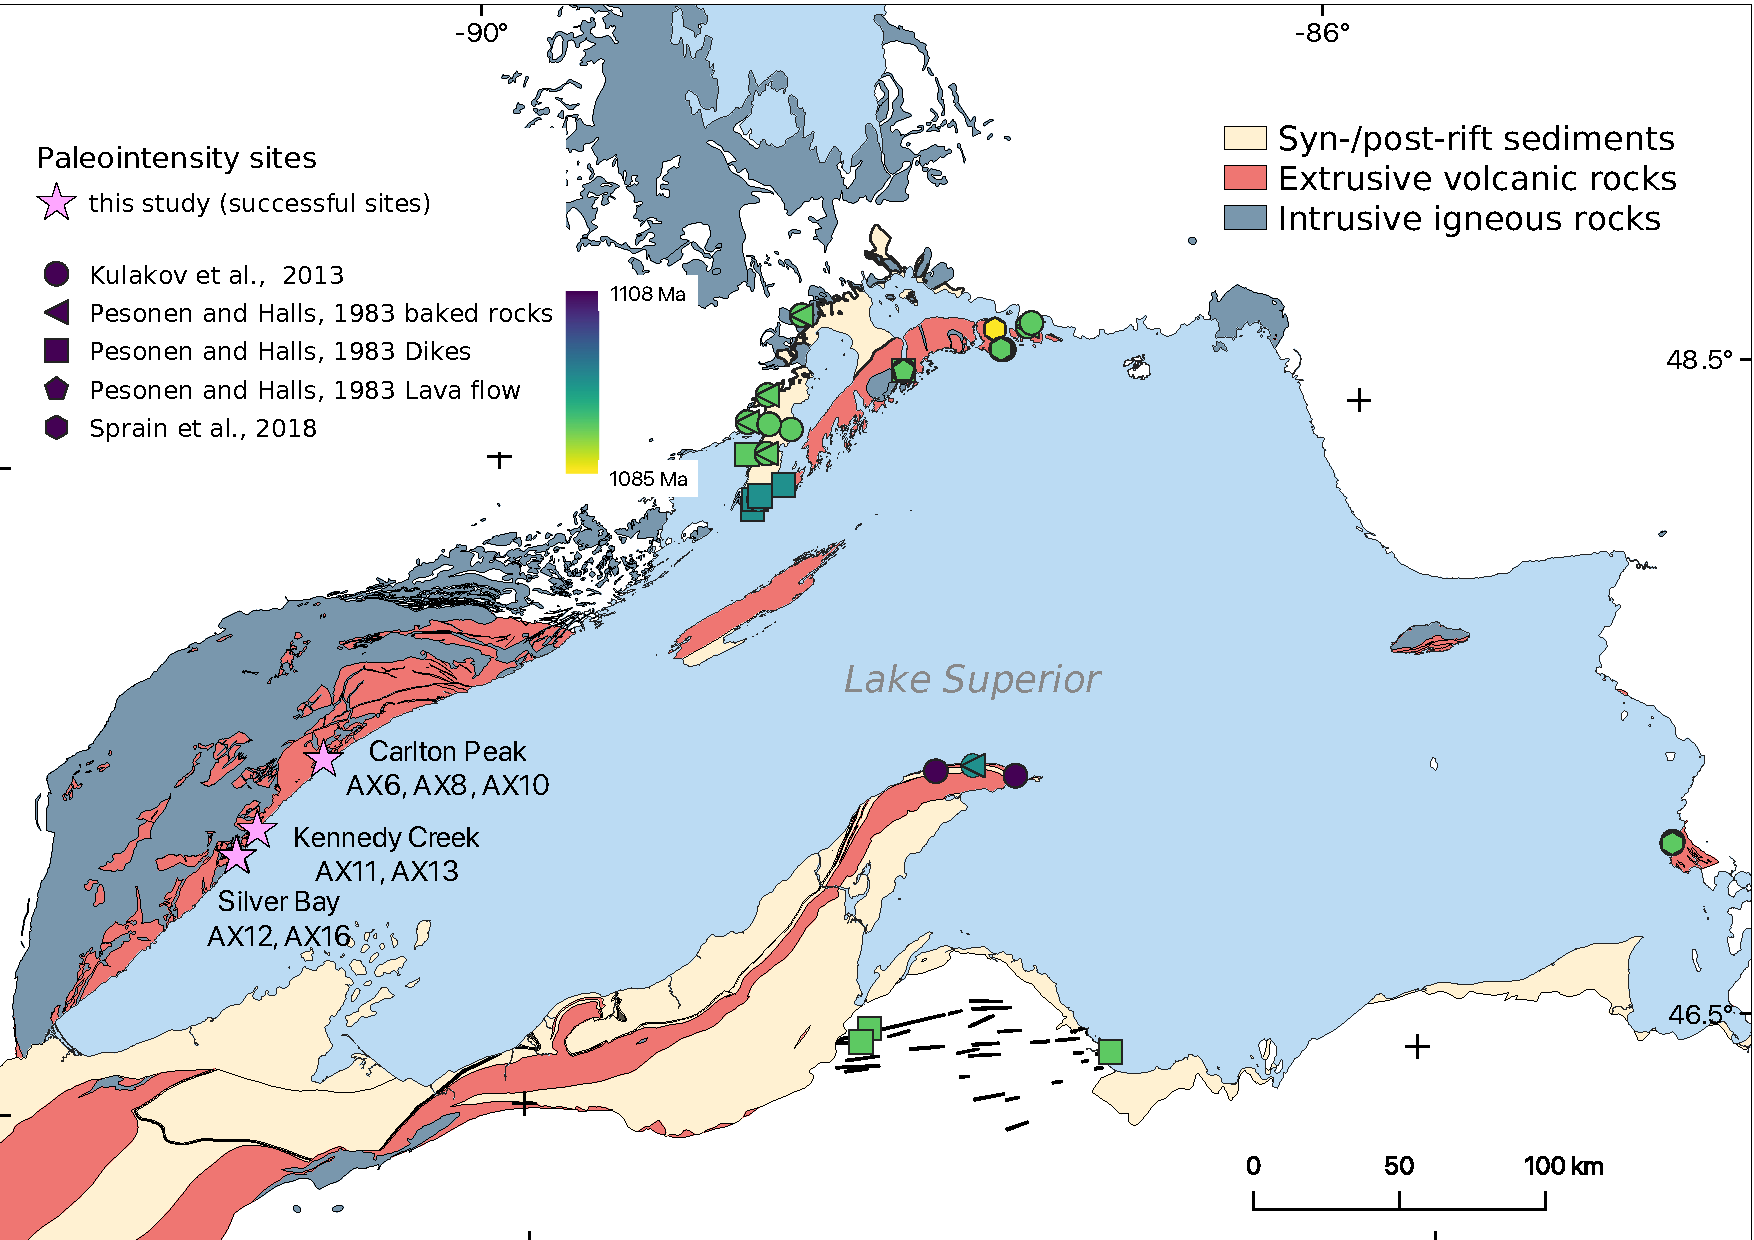
\includegraphics[width=11.4 cm]{Geologic_map.pdf}
\caption{\footnotesize{Simplified geologic map of the Lake Superior region showing the distribution of rift and post-rift-related rocks including extrusive, intrusive, and late/post-rift sediments around Lake Superior. Purple stars mark sites with paleointensity results that passed the selection criteria from this study. Paleomagnetic sites from  \citealp{Pesonen1983a} are categorized by lithology. All sites from  \citealp{Pesonen1983a, Kulakov2013a, Sprain2018a} are color-coded by their ages.}}
\label{fig:Geologic_map}
%\end{figure*}
\end{SCfigure*}

Determinations of the absolute value of ancient geomagnetic field strength rely on igneous rocks that acquire thermal remanent magnetizations as they cool. These magnetizations need to be unmodified by subsequent heating or chemical alteration in order to maintain a record of the ancient geomagnetic field from the time of cooling. Intracontinental magmatic events are therefore an important target for determination of ancient paleointensity as they can be well-preserved within continental interiors. This interior position results in them typically being distant from tectonic events along continental margins that can drive alteration through heat and fluids. However, intraplate magmatism associated with large igneous provinces is typically of geologically short duration with the bulk of magmatic products emplaced within 1 Myr or less \cite{Kasbohm2021a}. The Midcontinent Rift is an exception as it is a large igneous province where magmatism lasted $\sim$25 Myr from \texit{ca.} 1109 Ma to 1084 Ma \cite{Swanson-Hysell2019a}. Additionally, extension ceased in the Midcontinent Rift prior to lithospheric separation, preserving volcanic, intrusive, and sedimentary rocks of the rift within the continental interior. As a result, rocks of the rift have unusually simple paleomagnetic behavior for their greater than one billion-year-old age and paleomagnetic data from rift rocks forms a central record of Mesoproterozoic paleogeography \cite{Swanson-Hysell2021c}. The duration of magmatic activity within the Midcontinent Rift is longer than the entire 20.4 Myr long Neogene Period such that it enables an extended well-preserved window into the intensity of Earth's magnetic field in the late Mesoproterozoic. 

Despite the excellent preservation of the rocks, non-ideal paleointensity behaviors have challenged the interpretation of many previous paleointensity results from the Midcontinent Rift \cite{Pesonen1983a, Kulakov2013a, Sprain2018a}. The most trusted type of paleointensity estimate is that obtained through experiments in which the primary natural thermal remanent magnetization is progressively replaced by a laboratory magnetization that is imparted in a known field with internal consistency checks (such as in IZZI-style Thellier experiments;  \citealp{Yu2004a}). In such Thellier paleointensity experiments, one typical departure from ideal behavior is sagging or double-slopes as visualized in plots that show thermal remanent magnetization (TRM) acquired versus natural remanent magnetization (NRM) lost. For such data, distinct paleointensity estimates may be calculated depending on the interpreter's choice of slope. Typically, such non-ideal behavior would result in a higher paleointensity estimate from the steeper-sloped low-temperature portion and a lower paleointensity estimate from the high-temperature portion. For example, in data from the Midcontinent Rift,  \citealp{Pesonen1983a} used the low-temperature slope as the best representation of the past magnetic field strength (likely overestimating the field strength) whereas  \citealp{Kulakov2013a} used the high-temperature slope (likely underestimating the field strength). Results with such non-ideal behavior were rejected by \citealp{Sprain2018a} who applied stricter paleointensity selection criteria, but as a result had few accepted sites.

In this study, we target a unique rock type---high-purity anorthosite xenoliths. Anorthosites are cumulate rocks composed dominantly of the mineral plagioclase. They are attractive targets for paleomagnetic study as plagioclase crystals can enshroud minute magnetic inclusions from alteration with minor alteration of the plagioclase crystals not resulting in the formation of secondary iron oxides in contrast with mafic minerals such as olivine. The anorthosite xenoliths targeted in this study were brought to the near surface in magma that formed hypabyssal intrusions of the Beaver River diabase \cite{Zhang2021b}. They cooled and acquired their magnetizations in conjunction with the host diabase. Paleointensity experiments on the anorthosite xenoliths have a high success rate, yielding consistent specimen- and site-level paleointensity results. Rock magnetic data reveal that the anorthosite xenoliths have low anisotropy of thermal remanent magnetization (TRM) and can acquire TRM linearly within relevant field strengths. Magnetic imaging shows the anorthosite specimens have dominant magnetic carriers within and interstitial to plagioclase crystals, and they do not display strong preferred orientations. These single-slope, high quality paleointensity data, together with other high-quality paleointensity records during the protracted Midcontinent Rift magmatic activity, require that there was a strong late Mesoproterozoic geodynamo.

\section*{Anorthosite xenoliths of the Midcontinent diabase}

While magmatic activity within the Midcontinent Rift was protracted, there were intervals of particularly rapid volcanism and voluminous emplacement of intrusions. The ca. 1092 Ma Beaver Bay Complex in northern Minnesota punctuates one such period of magmatism during the main stage of Midcontinent Rift activity. The magma that formed the 1091.7 $\pm$ 0.2 Ma Beaver River diabase dikes and sills of the Beaver Bay Complex transported numerous anorthosite xenoliths that have short-axis diameters up to 180 meters via wide conduits \cite{Boerboom2004a, Boerboom2006b}. These anorthosite xenoliths are plagioclase cumulates that formed comagmatically with the host diabase in the lower crust---an interpretation confirmed by U-Pb zircon geochronology \cite{Zhang2021b}. 

Thermal modeling results and paleomagnetic directional data show the anorthosite xenoliths to have acquired thermal remanent magnetizations while cooling with the Beaver River diabase \cite{Zhang2021b}. Step-wise thermal demagnetization data show the anorthosite xenoliths to have dominantly single-component magnetization that often unblock sharply within temperature ranges between 500\textdegree C and 580\textdegree C, consistent with magnetization held by low-titanium titanomagnetite \cite{Zhang2021b}.

%\begin{figure*}
\begin{SCfigure*}
\centering
\noindent\includegraphics[width=13 cm]{Petro_QDM.png}
\caption{\footnotesize{Thin section petrographic images (A,B,C,D) and magnetic maps (E,F) of anorthosite from the Beaver River anorthosite xenolith from which paleomagnetic site AX16 and geochronology sample MS99033 were collected (left column;  \citealp{Zhang2021b}) and a distinct anorthosite from the Duluth Complex Anorthositic Series (right column). The Duluth Complex anorthosites were not targeted for paleointensity experiments in this study given the complexities associated with more pronounced fabrics. Cross-polarized petrographic images of the Beaver River anorthosite (A,C) reveal plagioclase with a granoblastic texture with crystals that are largely free of large opaque inclusions. In contrast, plagioclase crystals in the Duluth Complex anorthosite have euhedral, interlocking crystals with an igneous foliation (B) and the plagioclase crystals contain abundant Fe-Ti oxide needles that have preferred orientations that are often parallel with the [001] axis of the plagioclase. Magnetic field maps acquired with a quantum diamond microscope (QDM) show that the relatively weak magnetic sources within and interstitial to plagioclase crystals exist in the Beaver River anorthosite in (E) while large oxide needles within Duluth Complex plagioclase are strongly magnetic as evidenced through the overlapping magnetic fields above the oxides in (F). Magnetic field maps of (E) and (F) share the same spatial and magnetic scale. The unit of the axes are in $\mu$m.}}
\label{fig:Petro_QDM}
%\end{figure*}
\end{SCfigure*}

\section*{Results and Interpretations}

\subsection*{Petrography and magnetic imaging of anorthosite xenoliths}

The dominantly monomineralic anorthosite xenoliths within the Beaver River diabase often have granoblastic texture characterized by equigranular crystals with weakly developed petrofabrics (Fig. \ref{fig:Petro_QDM}A). In addition, the plagioclase crystals of the anorthosite xenoliths are typically free of large oxide inclusions (Fig. \ref{fig:Petro_QDM}C). Magnetic imaging using a quantum diamond microscope (QDM) shows that the dominant magnetic remanence carriers often exist within, and sometimes interstitial to, plagioclase crystals (Fig. \ref{fig:Petro_QDM}E). 

These features of the Beaver River anorthosite xenoliths are distinct from many other anorthosites such as the anorthosite xenoliths within the Duluth Complex Anorthositic Series rocks---older intrusions within the Midcontinent Rift. To illustrate these difference, we present petrographic and magnetic imaging data from a sample of Duluth Complex anorthosite that was not targeted for paleointensity experiments. The plagioclase of the Duluth Complex anorthosites typically develop interlocking textures that display strong igneous foliation (Fig. \ref{fig:Petro_QDM}B). In addition, there are abundant Fe-Ti oxide needles that are typically aligned with the [001] axes of the plagioclase crystals (Fig. \ref{fig:Petro_QDM}D). Magnetic imaging confirms that these strongly magnetic needles within the plagioclase crystals often have magnetic moments oriented along their long axes (Fig. \ref{fig:Petro_QDM}D,F). Titanomagnetite and ilmenite symplectic intergrowths also coexist with pyroxene and relict olivine as a product of olivine oxidation in the Duluth Complex magma \cite{Miller1990a}.

The lack of symplecites and the lack of large plagioclase-hosted titanomagnetite needles within the Beaver River anorthosite xenoliths distinguish them from plagioclase cumulates of the Duluth Complex and other layered mafic complex where anisotropic magnetic mineral fabrics associated with igneous foliation often occur \cite{Scofield1986a, Selkin2000a, Feinberg2006a}. The relative lack of fabric and associated preferred orientation makes the Beaver River anorthosite xenoliths a particularly compelling target for paleointensity experiments.

\subsection*{Paleointensity}

Following IZZI-modified paleointensity experiments \cite{Yu2004a}, 40 from a total of 86 anorthosite specimens and 0 out of a total of 69 diabase specimens passed our paleointensity result selection criteria (see Materials and Methods section). 7 anorthosite sites and no diabase site-level results pass these selection criteria. Example NRM/TRM (Arai) plots are shown in Fig. \ref{fig:IZZI_examples}. Summary specimen absolute paleointensity estimates and site-level weighted mean paleointensity values are plotted in Fig. \ref{fig:PINT_cooling_corrected} (and provided in Table S1). The paleointensity quality index (Q$_{PI}$;  \citealp{Biggin2014a}) for the anorthosite xenoliths are all 5 or 6 (Table S2). The cooling rate-corrected absolute paleointensity estimates from all anorthosite sites have a mean of 38.28 $\pm$ 11.92 $\mu$T. This paleointensity value corresponds to a calculated virtual dipole moment of $\sim$89 ZAm$^2$ ($10^{21} Am^2$) ca. 1092 Ma. All measurement-level paleointensity experiment data are available within the MagIC database (\url{https://earthorg/MagIC/19462/8d3c2258-11ae-4830-b99f-3f6b02eceb7e}; \textit{this private link is provided for the purpose of review; the url will be updated when a doi is generated for this manuscript}). 

\begin{figure*}
\noindent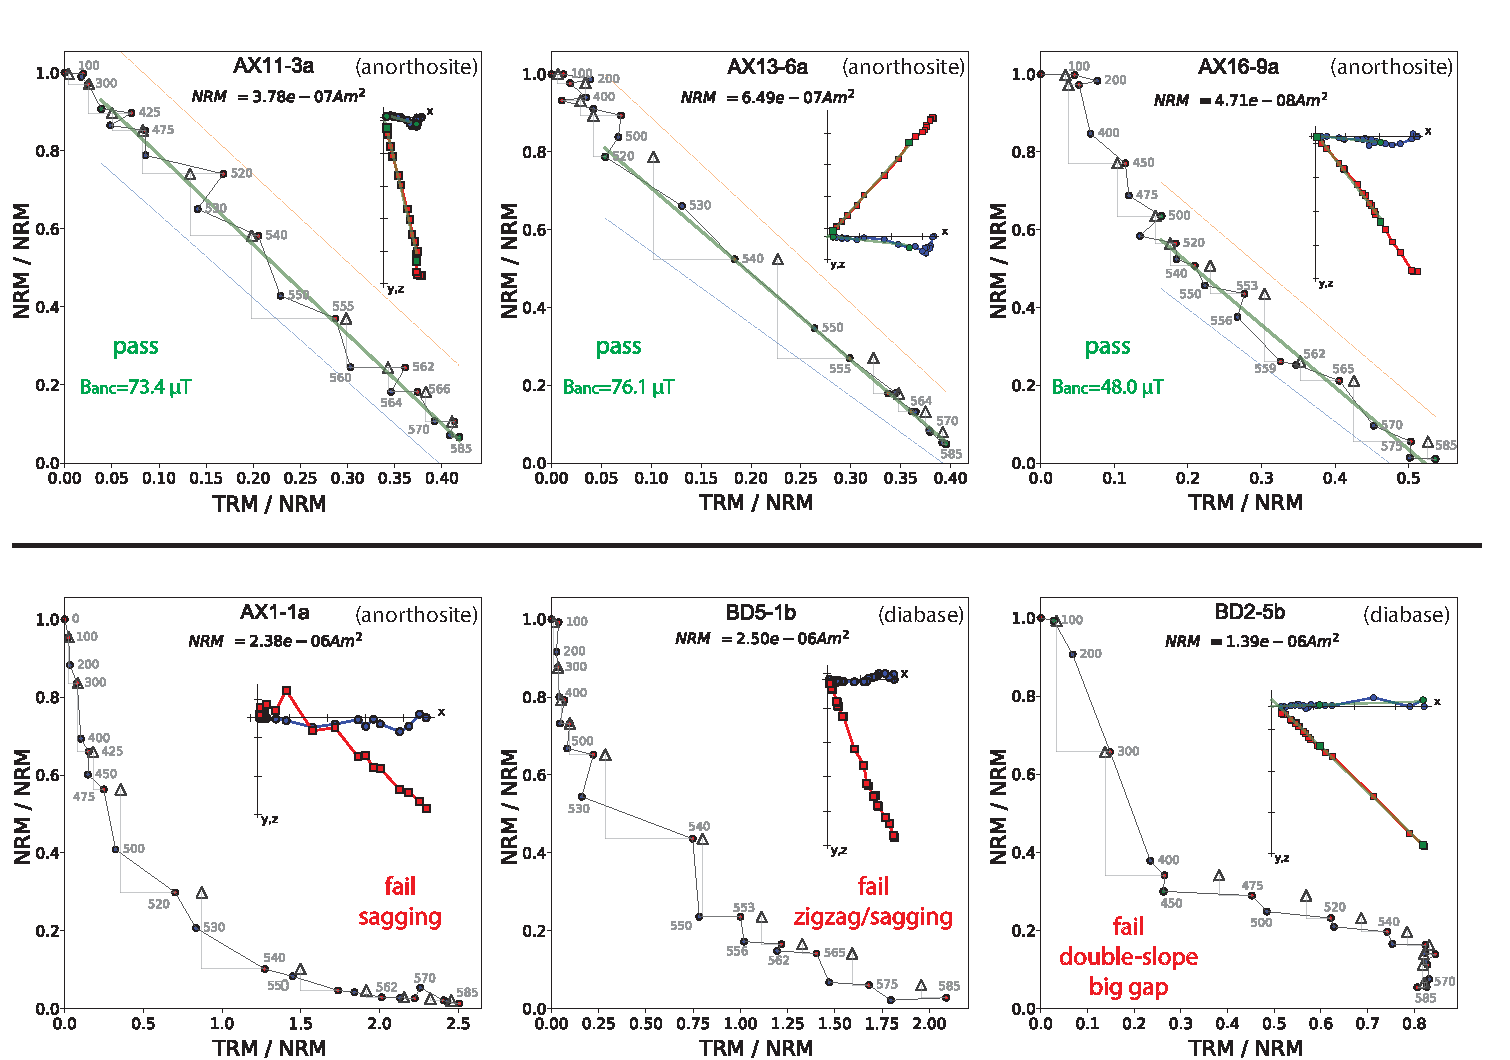
\includegraphics[width=17.8cm]{IZZI_examples.pdf}
\centering
\caption{\footnotesize{Example results of paleointensity experiments are displayed on Arai plots and zero-field heating results are shown on inset orthogonal plots (Zijderveld plots) for anorthosite and diabase specimens. Red (blue) circles indicate zero-field/in-field (in-field/zero-field) steps `ZI’ (`IZ’). Triangles mark partial thermal remanent magnetization (pTRM) checks. Blue and red squares in the Zijderveld plots are X–Y and X–Z projections, respectively, of the NRMs in specimen coordinates. Plots on the top row show successful specimen paleointensity results with straight, single-slope behaviors that pass our selection criteria. The green lines represent fits for the dominant single-slope component that passes the acceptance criteria and gives an estimate of the ancient field strength (B$_{anc}$). The plots for anorthosite specimens AX1-1a and diabase BD5-1b on the bottom row show typical non-ideal sagging behaviour that fails our acceptance criteria. Specimen BD2-5a is an example where the data appear linear with distinct slopes in the low and high temperature ranges such that it could pass less restrictive selection criteria, particularly if a narrower temperature range was used for the experiment.}}
\label{fig:IZZI_examples}
\end{figure*}

Typical paleointensity experimental data of the anorthosite specimens have straight, single-slope NRM/TRM plots and the accepted fractions of temperature steps span over the origin-trending, primary remanence components (Fig. \ref{fig:IZZI_examples}). We accept specimen- and site-level absolute paleointensity results from those anorthosite xenoliths that pass the selection criteria. Other anorthosite xenoliths and diabase specimens failed the selection criteria largely because of double-slope or sagging behavior (fail FRAC selection; see Materials and Methods section), poor pTRM checks, and sometimes zigzagging behaviors superimposed on top of sagging behavior (fail SCAT, DANG selection; see Materials and Methods section; Fig. \ref{fig:IZZI_examples}). A 20 mT alternating field treatment after in-field heating steps was applied to some specimens, but it did not result in significant changes in the experimental results for the anorthosite xenolith or diabase specimens (Fig. \ref{fig:PINT_cooling_corrected}; Supporting Information). 

\begin{figure*}[h!]
\noindent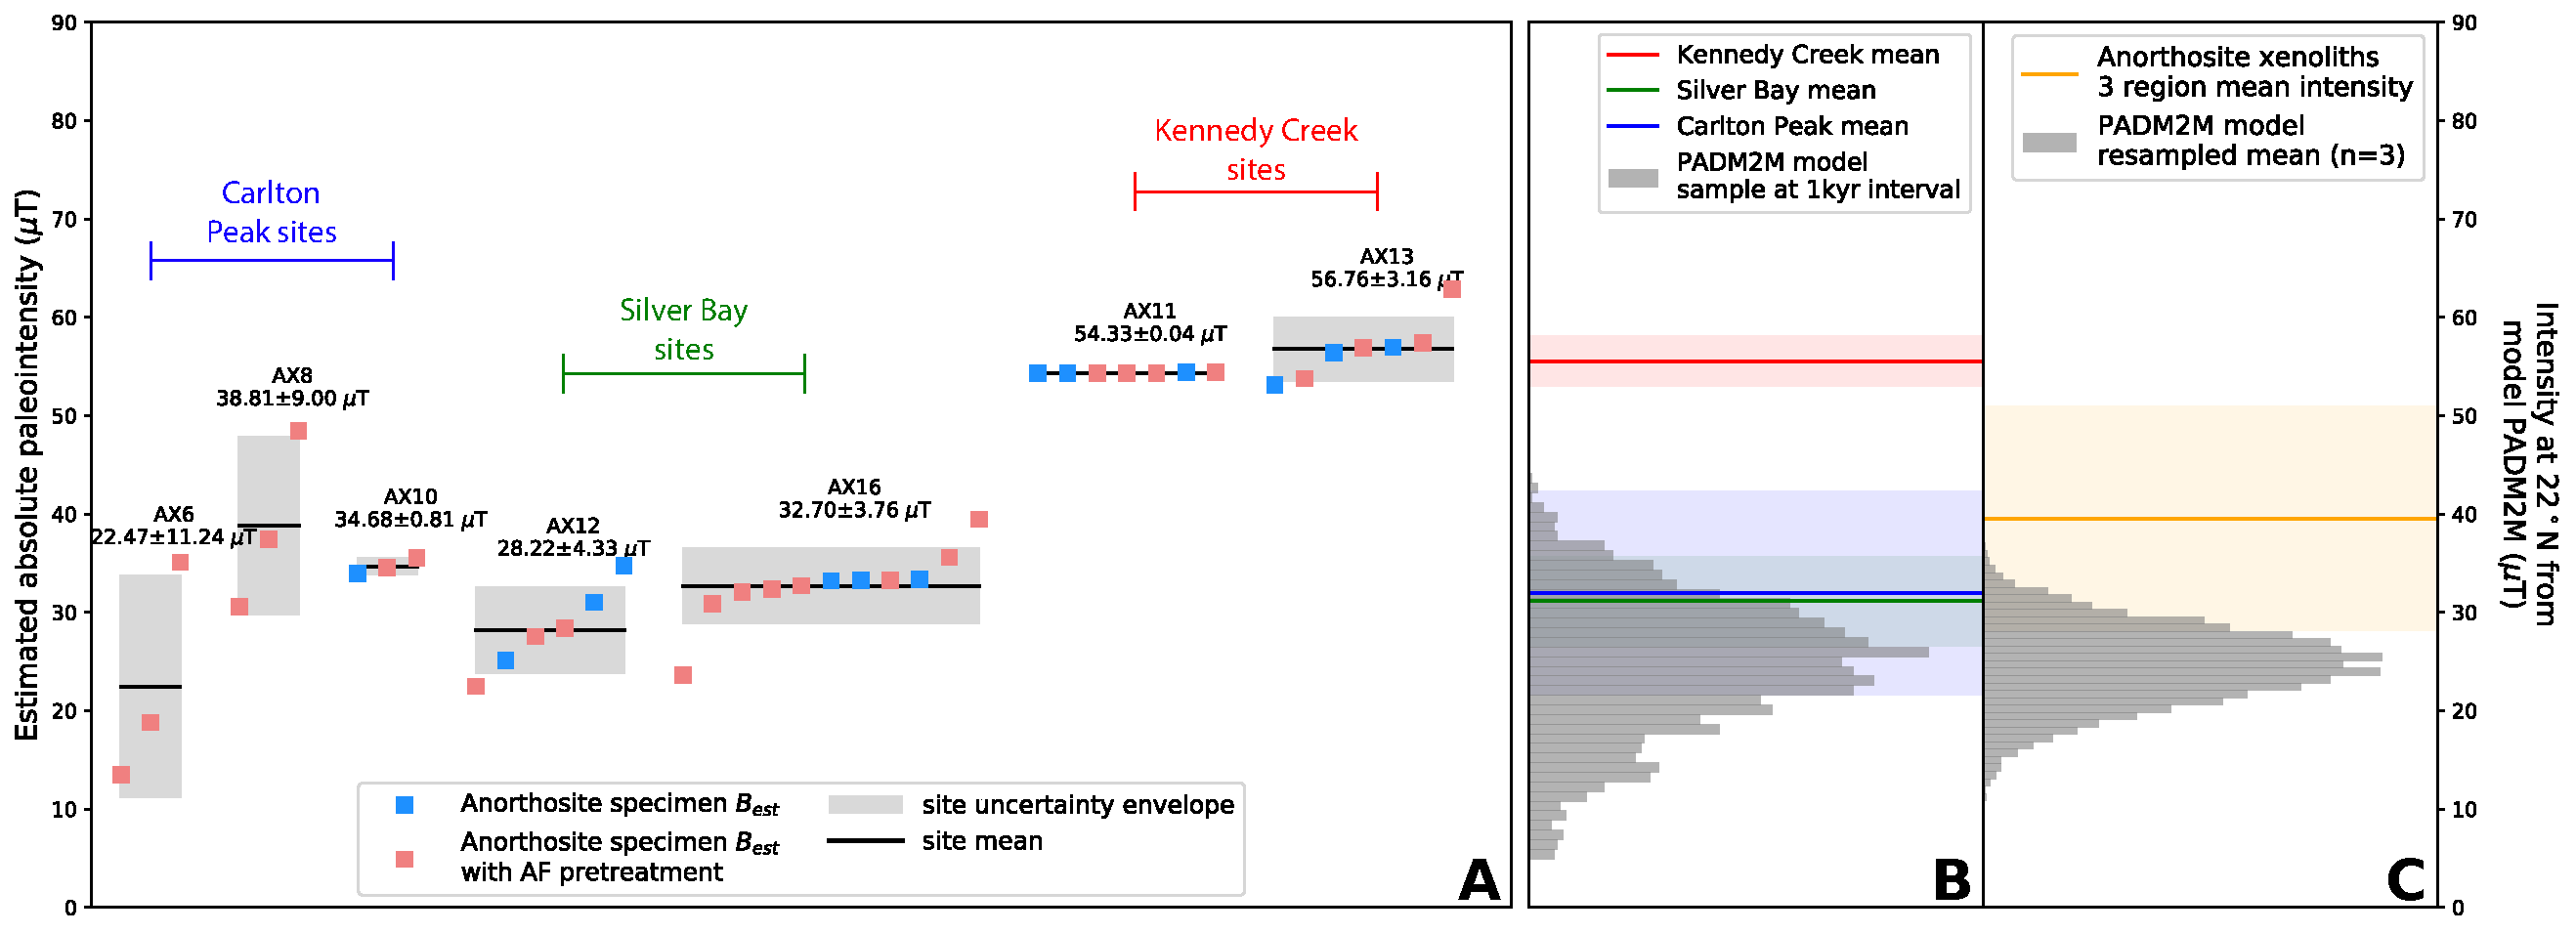
\includegraphics[width=17.8 cm]{Paleointensity_plot_cooling_corrected.pdf}
\centering
\caption{\small{Summary plot of individual specimen absolute paleointensity results (square symbols) from this study and their averages at site (black bars with grey uncertainty boxes) and locality level (weighted mean by site-level standard deviations; orange bar). All results are corrected for cooling rate with a factor of 0.74. }}
\label{fig:PINT_cooling_corrected}
\end{figure*}

In addition to estimating paleointensity values by introducing a set of selection criteria to filter our experiment results, we apply an independent method of \citealp{Cych2021a} which uses all experimental data regardless of their NRM/TRM plot statistics to perform bias corrected estimation of paleointensity (BiCEP). This Bayesian probabilistic method is based on an assumption that paleointensity estimates from specimens that come from a same cooling unit are distributed around a true paleointensity value with the various deflections being expressed as the curvature parameter of the NRM/TRM plot \cite{Paterson2011a}. The posterior paleointensity distributions from these sites with high-quality specimen-level data are in agreement with the site-level weighted-mean results developed using the selection criteria approach (Fig. \ref{fig:PINT_cooling_corrected}; Fig. S1).

Overall, the high-quality results from the anorthosite xenoliths of the Beaver River diabase and the consistent paleointensity estimates based on independent methods confirm that the anorthosite xenoliths record a high geomagnetic field ca. 1092 Ma. 

\subsection*{Rock magnetism}

Rock magnetic data support that the anorthosite specimens that pass the paleointensity selection criteria have dominant magnetic remanence carriers with magnetic properties similar to stochiometric, non-interacting, single domain magnetite, whereas anorthosite samples that failed the paleointensity result selection and all diabase samples have more pronounced populations of non-ideal carriers. Magnetic property measurement system (MPMS) data show both diabase and anorthosite contain (titano)magnetite as evidenced through the presence of the Verwey transition (Fig. S2;  \citealp{Verwey1939a, Feinberg2015a}). Anorthosite specimens from sites that yield successful paleointensity results have Verwey transition temperatures near 120 K as expected for stochiometric magnetite with minimal Ti \cite{Ozdemir1993a}. However, diabase and anorthosite specimens that did not pass our paleointensity selection typically have Verwey transitions that are suppressed toward lower temperatures (Fig. S2), indicating that magnetite grains in the specimens either have relatively higher Ti content or have been partially oxidized \cite{Ozdemir1993a}. 
 
Coercivity spectra from backfield experiments further support the interpretation that rocks that pass or fail the selection criteria have distinct magnetic mineralogy (Fig. \ref{fig:coercivity}). A compilation of median destructive field (MDF) values in Fig. \ref{fig:coercivity} shows that specimens from anorthosites that pass paleointensity selection criteria have distinctly higher average MDF values than other anorthosite and diabase specimens. Single-component fits for coercivity spectra \cite{Maxbauer2016a} show that anorthosites that yielded successful paleointensity results can have magnetic grain populations with peak coercivity around 80 mT (Fig. \ref{fig:coercivity}). In contrast, other anorthosite and diabase tend to have lower peak coercivities ($\sim$30 mT). This result is consistent with an interpretation that a population of magnetic grains with more multidomain-like behavior is responsible for the non-ideal paleointensity behaviors during experiments on such specimens.

\begin{figure}
\noindent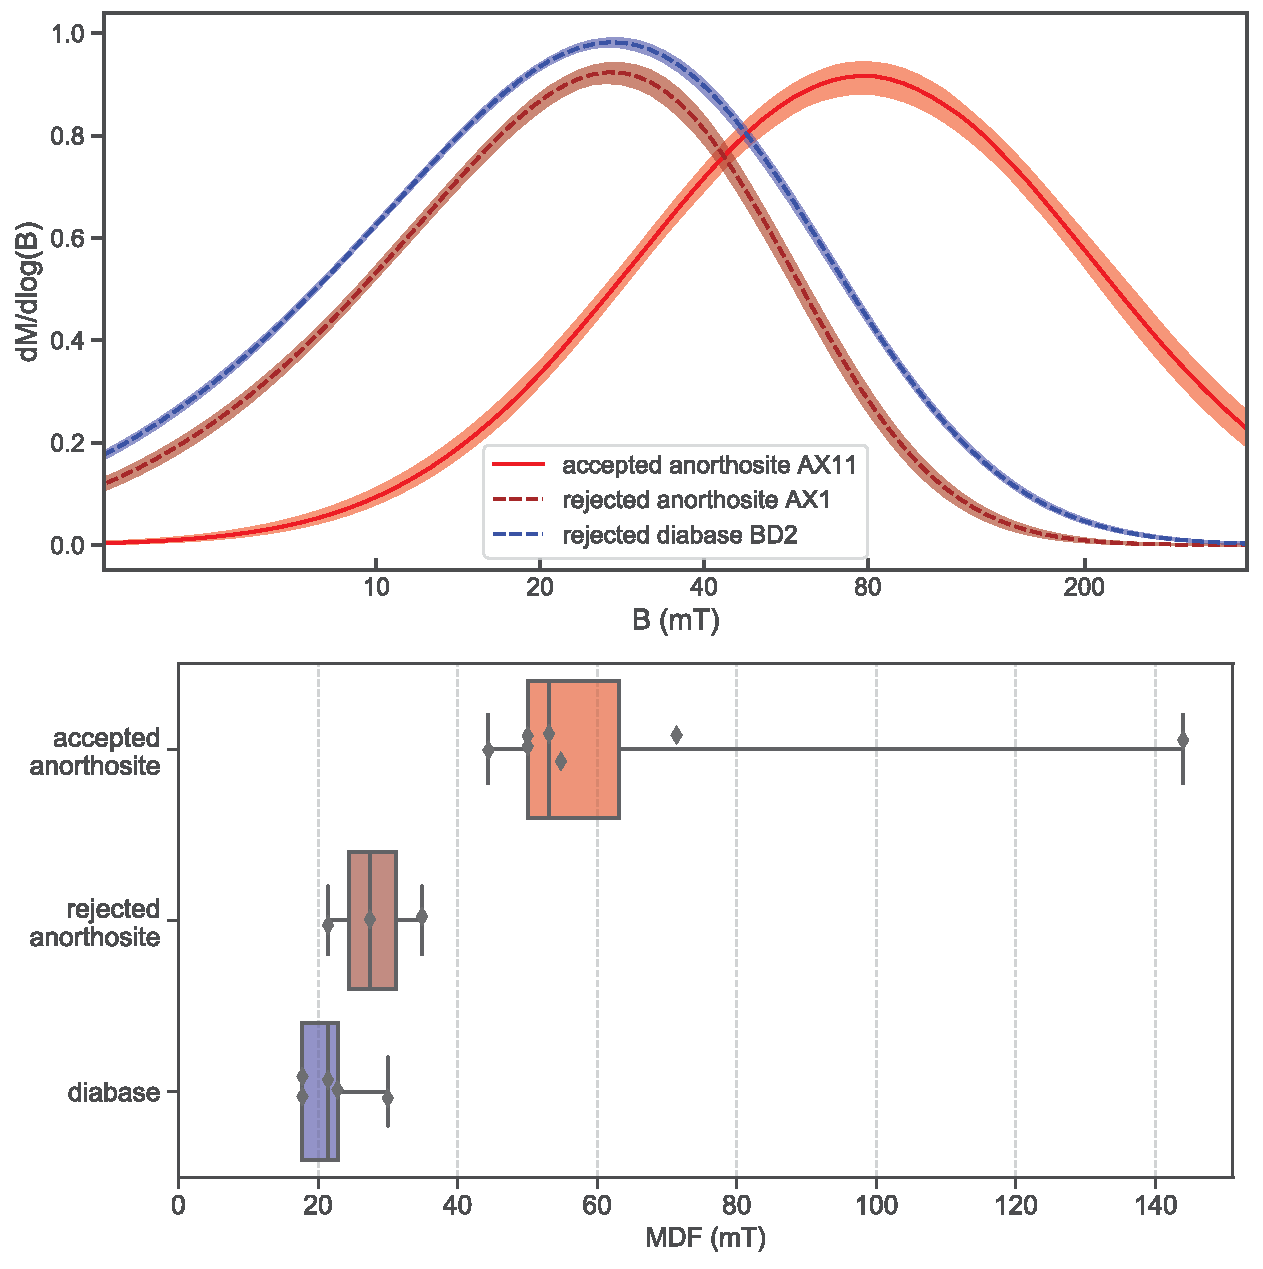
\includegraphics[width=\linewidth]{coercivity.pdf}
\centering
\caption{\footnotesize{Top: Example coercivity spectra of anorthosite and diabase specimens from sites that pass or fail our paleointensity selection criteria. Bottom: Box plots of median destructive field (MDF) values for all anorthosite and diabase specimens with single-component coercivity unmixing results. Both plots show that anorthosite specimens that pass paleointensity selection criteria have higher coercivities consistent with a higher portion of single-domain-like magnetite grains than the other anorthosite specimens and the diabase.}}
\label{fig:coercivity}
\end{figure}

\subsection*{TRM anisotropy and nonlinear acquisition check}
Significant remanence anisotropy has been documented to exist within certain anorthositic rocks that form in layered intrusive complexes \cite{Selkin2000a, Feinberg2006a}. Strong remanence anisotropy associated with the igneous foliation developed within anorthosite from the Stillwater Complex has been shown to lead to significant overestimation or underestimation of paleointensity values depending on the relative orientations between the fabrics and an applied magnetic field \cite{Selkin2000a}. To assess whether our paleointensity estimates are biased by remanence anisotropy, we calculated the gamma statistic, which is the angular difference between the last pTRM step of paleointensity experiment and the applied field direction. The results show that the anorthosite specimens used for paleointensity experiment have low gamma values ranging from $\sim$0.9\textdegree to $\sim$11.9\textdegree, with a median value of 4.2\textdegree$\;$(Table S1). These gamma values are similar to those of Midcontinent Rift volcanics \cite{Sprain2018a}. Therefore, the Beaver River anorthosite xenolith bulk samples do not have a significant remanence anisotropy. Paleodirectional data from our anorthosite xenoliths further support that they have minimal remanence anisotropy as their site mean directions closely match those of the Beaver River diabase hosts without deviating due to a fabric \cite{Zhang2021b}. In addition, no resolvable magnetic fabric was observed in the anorthosite xenoliths through petrographic and magnetic imaging (Fig. \ref{fig:Petro_QDM}). 

We applied full TRMs to a set of anorthosite specimens with lab fields of 30, 50, 70, and 90 $\mu$T along specimen vertical axes. The results show that our anorthosite specimens did not saturate upon the applied fields and there is thus no need for correcting nonlinear thermal remanence acquisitions ( \citealp{Selkin2007a}; Fig. S4). 

\subsection*{Averaging secular variations and applying cooling rate correction}
To best characterize the geomagnetic axial dipole field intensity during a certain time period a paleointensity dataset should cover a sufficient amount of time such that paleosecular variations of the geomagnetic field are averaged. Thermal modeling results from \citealp{Zhang2021b} suggest that the Beaver River anorthosite xenoliths were heated to tholeiitic magma temperature ($\sim$1100\textdegree C) and acquired thermal remanent magnetization during cooling with their diabase host on a time scale of a thousand years, partially averaging secular variation within single samples. Anorthosite xenoliths have paleointensity results that are consistent within small regions, but vary between localities. Anorthosite AX12 and AX16 were emplaced $\sim$450 meters apart and have very similar paleointensity estimates (Fig. \ref{fig:Geologic_map, fig:PINT_cooling_corrected}). $\sim$10 km to the north, anorthosite xenoliths AX11 and AX13 were also emplaced closely at a distance of $\sim$125 meters and yield similar but distinct paleointensity estimates from those of AX12 and AX16 (Fig. \ref{fig:Geologic_map, fig:PINT_cooling_corrected}). The data therefore capture different intervals of time during the emplacement and cooling of the Beaver River diabase sills ca. 1092 Ma. 

Another consequence of the anorthosite xenoliths having cooled in the interior of thick diabase intrusions is that slow cooling rates can bias paleointensity estimates toward higher values. Large differences in cooling rates between acquisition of an NRM in nature versus a TRM in the lab can result in overestimated paleointensities for SD grains \cite{Dodson1980a, Halgedahl1980a, Nagy2021a}. From the thermal history model of  \citealp{Zhang2021b}, we can estimate the duration over which the diabase and anorthosite cooled from the Curie temperature of magnetite ($\sim$580\textdegree C) to the time when they fully blocked in their characteristic natural remanence magnetization ($\sim$500\textdegree C;  \citealp{Zhang2021b}). We find the cooling time to be on the order of $\sim$1 kyr, which corresponds to a cooling rate of $\sim1.6\times10^{-9}$ $^\circ$C s$^{-1}$. In contrast, the lab cooling rate is much faster through the same temperature interval with an estimated cooling rate of $\sim1.3\times10^{-1}$ $^\circ$C s$^{-1}$. The significant cooling rate difference leads to a predicted $\sim$36\% overestimate of true ancient field following the model of \citealp{Halgedahl1980a} (Fig. S3). This estimate on cooling rate effect is similar to the value of $\sim$35\% overestimate derived from the model of \citealp{Nagy2021a}. We therefore correct our paleointensity results by a factor of 0.74. The cooling rate-corrected specimen paleointensity estimates together with specimen- and site-level weighted means are shown in Fig. \ref{fig:PINT_cooling_corrected}.


\begin{figure*}[h!]
\noindent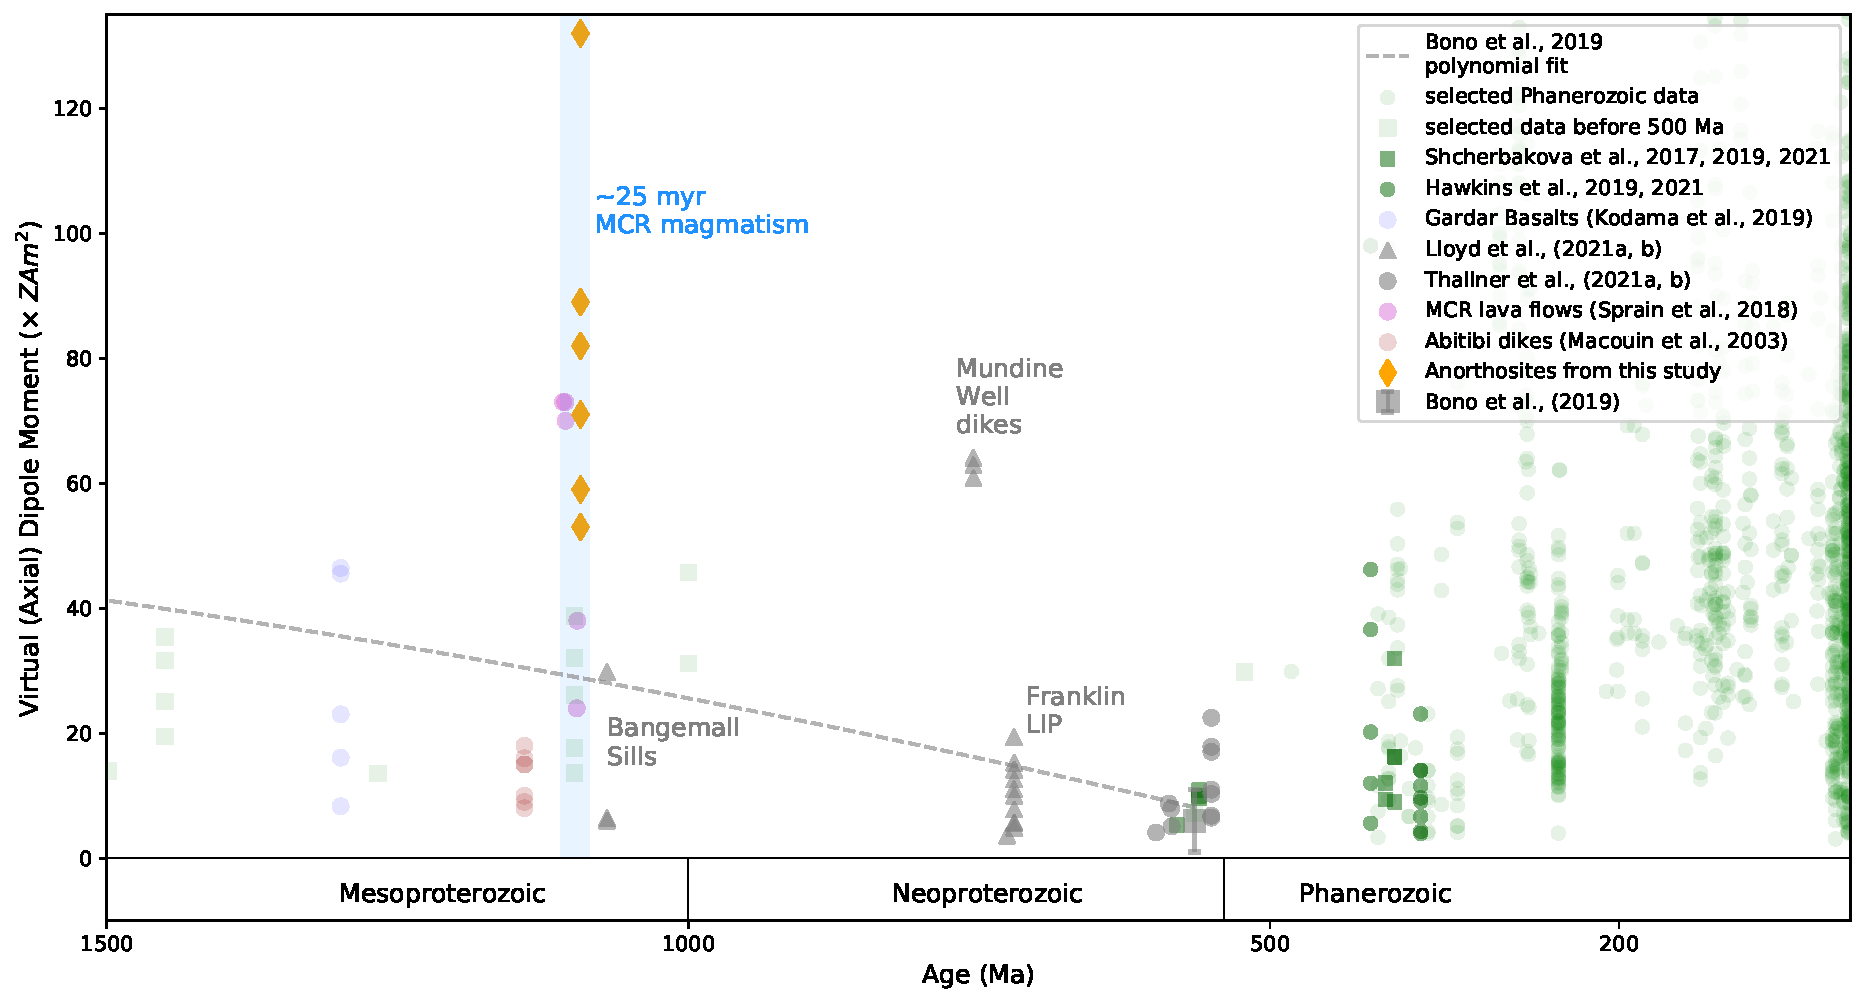
\includegraphics[width=17.8 cm]{PINT_compilation.pdf}
\centering
\caption{\footnotesize{Compilation of calculated virtual (axial) dipole moment values from the PINT database (PINT v8.0.0; \url{http://www.pintdb.org/};  \citealp{Bono2021a}) with additional Neoproterozoic data from refs. \citealp{Lloyd2021a, Lloyd2021b, Thallner2021a, Thallner2021b}. Paleointensity estimates from \cite{Pesonen1983a} and \cite{Kulakov2013a} are not included in the compilation due to the specimen-level double-slope behavior as discussed in the text. Overall the anorthosite xenoliths from this study record a high Mesoproterozoic field exceeding the value projected by the second order polynomial curve from \cite{Bono2019a} which is based on an interpretation of there being a monotonic decay of the geodynamo through the Proterozoic.}}
\label{fig:PINT_compilation}
\end{figure*}

\section*{Discussion}

%The outline for this section is::
%- Discussion of mineral physics constraints (or lack thereof)
%- Predictions for paleointensity signal associated with inner core nucleation (or lack thereof)
%- Interpretations of paleomagnetic record (i.e. Bono model of monotonic decrease and then rapid increase;. Cite Biggin et al. 2015) related to inner core nucleation. 
%- Challenges posed to this model based on our data and other low to strong field transitions.

The crystallization of the solid inner core is an important event in the long-term evolution of Earth's core and in sustaining the geodynamo \cite{Buffett2000a}. The age of the inner core in thermal evolution models relies on estimates for the thermal conductivity of iron alloys at the temperatures and pressures of the core \cite{Ohta2021a}. Prior to studies in the last 10 years, an accepted value of $\sim$30 W m$^{-1}$ K$^{-1}$ for this thermal conductivity was used to constrain the timing of inner core nucleation to be during the first half of Earth history \cite{Stacey2007a, Konopkova2016a}. Subsequently, experimental data and \textit{ab intio} simulations were interpreted to imply higher thermal conductivity values \cite{Pozzo2012a, Ohta2016a} which in turn imply a younger age of the inner core ($<$700 Ma; \citealp{Labrosse2015a}). However, other experimental studies continue to indicate lower thermal conductivity values consistent with prior estimates \cite{Konopkova2016a, Hsieh2020a} with no consensus yet emerging \cite{Williams2018a, Ohta2021a}. These experiments are challenging with issues such as constraining the sample thickness under high pressure and temperature conditions, the validity of applying the Wiedemann-Franz law to extrapolate thermal conductivity values based on electrical resistivity measurements \cite{Ohta2016a}, and modeling uncertainties associated with parameters used in direct thermal conduction measurement experiments \cite{Konopkova2016a}. Further experiments and theory are needed to explain these contrasting results which at present leave open very different trajectories for Earth's thermal evolution. As a result, the age of the inner core is relatively unconstrained from a theoretical perspective. 

The other data type that can provide insight into the long-term history of the core's thermal regime and geodynamo is paleomagnetic data---both paleodirectional data that indicate the presence of a geomagnetic field and paleointensity data that constrain the field's strength. Inner core nucleation would have increased the power to the geodynamo which has the potential to manifest as an increase in Earth's surface field \cite{Davies2021a}. An approach combining dynamo simulations and power-based theoretical scaling relationships has predicted that progressive decay of the field's dipole moment would be followed by a rapid increase in geomagnetic field intensity soon after the onset of inner core nucleation such that there is a minimum in dipole moment just before inner core nucleation \cite{Davies2021a}. Other scenarios are possible, however, such as the prediction that while power increases associated with inner core nucleation would result in increases in Earth's internal magnetic field strength, the dynamo would also become more deeply seated in the core, diminishing the increase in observed magnetic field at Earth's surface \cite{Aubert2009a, Landeau2017a}. Observational paleomagnetic records hold the potential for testing different model predictions and identifying transitions in ancient field strength.

It has been proposed that Proterozoic paleointensity data are consistent with a progressive monotonic decay leading up to ca. 565 Ma in the Ediacaran Period (Fig. \ref{fig:PINT_compilation}, \citealp{Bono2019a}). This interpretation was motivated by paleointensity estimates developed from the ca. 565 Ma Sept-$\hat{I}$les layered mafic intrusive complex of $\sim$7 ZAm$^2$ that are among the lowest values in the paleointensity database (Fig. \ref{fig:PINT_compilation}), \citealp{Bono2019a}. A decay in the lead-up to this time was argued to be consistent with an absence of an inner core and a dynamo to which progressively less power was available through secular cooling \cite{Bono2019a, Davies2021a}. This timing of inner core formation would favor a high core thermal conductivity \cite[e.g.][]{Ohta2016a}. Paleomagnetic directional excursions \cite{Halls2015a} and frequent polarity reversals \cite{Kodama2021a} during this time are interpreted to be consistent with numerical simulations \cite{Driscoll2016a} associated with a weak dipole field. 

The high paleointensity estimates from the Midcontinent Rift rocks challenge the hypothesized monotonic decay of the strength of the geomagnetic field throughout the Proterozoic Era. Instead, the well-preserved ca. 1092 Ma anorthosite xenoliths of the Beaver River diabase record a strong geomagnetic field in the late Mesoproterozoic that exceeds the strength of the modern-day field for which crystallization of the inner core is a power source (Fig. \ref{fig:PINT_compilation}). Together with previous records obtained from the ca. 1106 Ma Osler Volcanics of the Midcontinent Rift \cite{Sprain2018a}, these data indicate that appreciable power to Earth's dynamo persisted through at least 14 Myr during the late Mesoproterozoic to maintain a strong surface field (Fig. \ref{fig:PINT_compilation}). In addition to these high geomagnetic fields recorded by Midcontinent Rift rocks, the ca. 755 Ma Mundine Well dikes \cite{Lloyd2021b} also require a stronger geomagnetic field in the Neoproterozoic than would be predict by a progressive Proterozoic decline (Fig. \ref{fig:PINT_compilation}). 

The hypothesis that a weak Ediacaran geomagnetic field is a telltale sign of the lack of an inner core with core nucleation following shortly thereafter may predict that it is the most significant weak to strong field transition in the paleointensity record. However, Fig. \ref{fig:PINT_compilation} shows that transitions from low to high field intensities occurred before, during, and after the Ediacaran. In the Ediacaran record developed to date, there is a two-fold increase in Earth's virtual dipole moment when comparing estimates from the ca. 565 Ma Sept-$\hat{I}$les intrusions \cite{Bono2019a} to those from ca. 550 Ma volcanics of the Skinner Cove Formation \cite{Thallner2021a} (Fig. \ref{fig:PINT_compilation}). In the late Mesoproterozoic, there is at least a six-fold increase within a period of $\sim$40 Myr from a low average virtual dipole moment of $\sim$13 ZAm$^2$ recorded by the ca. 1140 Ma Abitibi dikes which yielded straight Arai plots \cite{Macouin2003a}, to a high moment of $\sim$70 ZAm$^2$ recorded by the ca. 1106 Ma Osler Volcanics, with even stronger values recorded ca. 1092 Ma by Beaver River anorthosite xenoliths that record virtual dipole moments up to $\sim$140 ZAm$^2$. While the Abitibi dikes paleointensity estimates do not go to values as low as the Sept-$\hat{I}$les intrusions, this virtual dipole moment increase in the Mesoproterozoic is the largest yet documented in the Precambrian (Fig. \ref{fig:PINT_compilation}). The tempo and scale of this field intensity transition could match with model-based predictions associated with the onset of inner core nucleation \cite{Davies2021a}. This timing would be broadly consistent with that proposed by \citealp{Biggin2015a}. However, the model prediction would be of sustained strong field values following inner core nucleation which is challenged by data from the ca. 1070 Ma Bangemall Sills which include a sill with a low virtual dipole moment of $\sim$6.4 ZAm$^2$ (Fig. \ref{fig:PINT_compilation};  \citealp{Lloyd2021b}). Following the Ediacaran, there are low paleointensity estimates from the ca. 414 Ma Strathmore lava flows \cite{Hawkins2021a}, the ca. 410-380 Ma lava flows of the Minusa Basinand the Kola Peninsula \cite{Shcherbakova2017a}, the ca. 408–393 Ma Buribay volcanic complex \cite{Shcherbakova2021a}, as well as the ca. 370 Ma dikes and lavas of the Siberian Viluy Traps \cite{Hawkins2019a} (Fig. \ref{fig:PINT_compilation}). This interval of time with low paleointensity estimates has been termed the ``Mid-Paleozoic Dipole Low'' \cite{Hawkins2021a} and is followed by high paleointensity values afterwards (Fig. \ref{fig:PINT_compilation}). 

% that represent a transition to field strengths greater than the present

% changes in core-mantle boundary heat flow related to plate tectonics - more general refrence to core-mantle heat flow pattern not necessarily telling about inner core nucleation. 

An alternative hypothesis for the multiple transitions from low to high field intensities in the middle Paleozoic and the Proterozoic is that they are manifestations of secularly changing mantle forcing of the geodynamo across the core–mantle boundary which may be unrelated to the growth of the inner core. The time scale over which these changes happen may be on the order of less than one million years. During the Pleistocene, when we known a present-day-like geodynamo existed, paleointensity records show at least a six-fold fluctuation of the geomagnetic dipole moment can happen (Fig. \ref{fig:PINT_compilation}). If the mantle forcing that drove such transitions exists regardless of the present of inner core, it could have contributed to the anomalously low or high paleointensity values observed during the Phanerozoic and Proterozoic. The low paleointensity records from the ca. 720 Ma dolerite dikes of the rapidly emplaced Franklin Large Igneous Province could be one example of capturing these short-term variations and not fully averaging the secular changes of the geomagnetic field (Fig. \ref{fig:PINT_compilation}; \citealp{Lloyd2021a, Lloyd2021b}). The unknown magnitude of the forcing presents challenges for detecting the increase in dynamo strength caused by the kick-start of compositional convection driven by the crystallization of the inner core based on paleointensity data alone. 

% This interpretation may explain the low virtual dipole moment of 11 ZAm$^2$ recorded by the ca. 

Overall, the high-fidelity paleointensity recorders of the Beaver River anorthosite xenoliths in the well-preserved Midcontinent Rift record high paleointensities values and necessitates that there was a vigorous late Mesoproterozoic geodynamo. 

% In the Neoproterozoic, ca. 720 Ma dolerite dikes of the Franklin Large Igneous Province record a mean virtual dipole moment of  In the Phanerozoic, multiple low paleointensities has been observed in Devonian-aged volcanic units (Fig. \ref{fig:PINT_compilation}; \citealp{Shcherbakova2017a, Shcherbakova2021a, Hawkins2021a}). 

%The observed paleointensity variations from the Midcontinent Rift also question the attribution to the onset of inner core nucleation as the unique cause for driving a significant paleointensity increase.  Besides the

% Accompanying the low paleointensity values, paleodirectional data from the Ediacaran-Cambrian \cite{Bono2015a, Halls2015b, Kodama2021a} and the Devonian show anomalous directional fluctuations \cite{Shcherbakova2019a} which could be consistent with there being a largely diminished dipole component of Earth's magnetic field. If the weak paleointensities in the Ediacaran or the Devonian are attributed to the geodynamo being on the brink of collapse just prior to the nucleation of the solid inner core. 

% rocks from 

% if one invokes inner core nucleation for all these low to high transitions, the data would suggest the inner core nucleated multiple times. Alternatively, it could that all except one are not related to the inner core nucleation, but merely a manifestation of short term dynamo variations. 
% n narrow time scales regardless of the existence of a solid inner core. Therefore, low paleointensity values or short-term fluctuations may not be sufficient evidence for interpreting Earth's inner core status through history.

% The high geomagnetic field estimates from the Midcontinent Rift volcanics and intrusives are not the only suite of high paleointensity records at odds with the hypothesis of a monotonically decaying geodynamo through the entire Proterozoic Eon \cite{Biggin2009a, Bono2019a}. The $\sim$60 ZAm$^2$ virtual dipole moment estimates from the ca. 755 Ma Mundine Well dikes are much higher than the values predicted by the monotonic decrease model of \cite{Bono2019a}. Although one may consider these data capturing relatively short term fluctuations of the geomagnetic field, they nevertheless indicate that the geodynamo had strong power sources during the Proterozoic. On the other hand, besides the low paleointensity values recorded by the ca. 1140 Ma Abitibi dikes, low estimates have been obtained from the ca. 1070 Ma Bangemall Sills \cite{Lloyd2021b}, the ca. 720 Ma dolerite dikes of the Franklin Large Igneous Province \cite{Lloyd2021a}, as well as Devonian-aged rocks from the Minusa Basin, Kola Peninsula, Buribay volcanic complex and volcanic rocks from the East European Craton (Fig. \ref{fig:PINT_compilation};  \citealp{Shcherbakova2017a, Shcherbakova2019a, Shcherbakova2021a}). The multiple occurrences of low geomagnetic field intensities during the Proterozoic and the Paleozoic indicate that a waning thermal convection regime in Earth's before the emergence of the solid inner core may not be the solely possible mechanism for triggering an weak dipole field. 


% In the meantime, paleomagnetic directional anomalies may be another suite of intriguing observational records that is worth investigating. The anomalous directional fluctuations during the Ediacaran and Devonian \cite{Bono2015a, Kodama2021a, Shcherbakova2019a} perhaps can be consistent with there being a weak geodynamo regime when dipole component of Earth's field was largely diminished. 



% conclude on whether an apparent rise or decay within a narrow time period ($\sim$35 Ma) during the Proterozoic is associated with transitions in the core phase transition or is a result of short-term excursion of the geomagnetic field that may be common through much of the evolution of Earth's core.

% an apparent rapid decrease in geomagnetic dipole moment from ca. 1092 Ma to ca. 1070 Ma can be evidenced by the contrasting high values from the Midcontinent Rift anorthosite xenoliths and the low values from the Bangemall Sills (Fig. \ref{fig:PINT_compilation};  \citealp{Lloyd2021b}). These data suggest that an apparent transition of virtual dipole moment similar in scale with what is predicted for a dynamo powered with or without compositional convection in the core may not be unique during the Precambrian. In addition, given that a five-fold fluctuation of the geomagnetic dipole moment exist in the paleointensity records for the past 10 million years, when we know a modern-day-like geodynamo likely powered by both thermal and compositional convection existed, we cannot conclude on whether an apparent rise or decay within a narrow time period ($\sim$35 Ma) during the Proterozoic is associated with transitions in the core phase transition or is a result of short-term excursion of the geomagnetic field that may be common through much of the evolution of Earth's core. Recently, ultra-low paleointensities (2.01–7.07) $\mu$T from the Devonian has been found by  \cite{Shcherbakova2021a}. These data suggest that significant excursion of low geomagnetic field intensities may occur regardless of the inner core formation. 

% These data suggest that an apparent transition of virtual dipole moment similar in scale with what is predicted for a dynamo powered with or without compositional convection in the core may not be unique during the Precambrian. In addition, given that a five-fold fluctuation of the geomagnetic dipole moment exist in the paleointensity records for the past 10 million years, when we know a modern-day-like geodynamo likely powered by both thermal and compositional convection existed, we cannot conclude on whether an apparent rise or decay within a narrow time period ($\sim$35 Ma) during the Proterozoic is associated with transitions in the core phase transition or is a result of short-term excursion of the geomagnetic field that may be common through much of the evolution of Earth's core. 



% Paleomagnetic observational records near the Ediacaran-Cambrian boundary have been interpreted to be consistent with a trend of decreasing axial dipole strength toward a very low value \cite{Lloyd2021a, Bono2019a}, followed by a rapid recovery (a few tens of million years) toward higher values soon after \cite{Thallner2021a}. Such a decrease-increase transition can be consistent with dynamo numerical simulations which adopt a rather high thermal conductivity of the core and projects an inner core birth near this time \cite{Gomi2013a, Davies2015a, Labrosse2015a, Ohta2016a}. In particular, some models have suggested that the kick-start of rigorous compositional convection between the inner core and the outer core due to the onset of inner core nucleation can result in almost an order of magnitude increase in Earth's axial dipole moment \cite[e.g.][]{Davies2021a}. The enriching observational records from the Ediacaran and Cambrian have been suggested to indicate that a geodynamo driven solely by thermal convection was waning to its brink of collapse near the end of Ediacaran \cite{Bono2019a, Thallner2021b} and was recovering toward modern-day strengths in the Cambrian \cite{Thallner2021a}.

% However, the updated paleointensity records from the Midcontinent Rift together with previous results from other Mesoproterozoic rocks suggest that the a dramatic increase in geomagnetic dipole moment similar in scale to that modeled for after the onset of inner core nucleation may not be unique to the Ediacaran-Cambrian boundary (Fig. \ref{fig:PINT_compilation}). The ca. 1140 Ma Abitibi dikes \cite{Macouin2003a} record an average virtual dipole moment of $\sim$13 ZAm$^2$, similar to the low values of $\sim$7 ZAm$^2$ obtained from the single silicate crystals of the ca. 565 Ma Sept-$\hat{I}$les intrusions \cite{Bono2019a}. However, the relatively high moments of $\sim$72 ZAm$^2$ from the ca. 1105 Ma Osler Volcanic Group \cite{Sprain2018a} and $\sim$89 ZAm$^2$ from the ca. 1092 Ma Beaver River anorthosite xenoliths (Fig. \ref{fig:PINT_compilation}) are about six times the values from the Abitibi dikes. This increase in absolute dipole moment estimates during $\sim$50 Myr recorded by the Midcontinent Rift rocks are much higher than that in the Ediacaran (Fig. \ref{fig:PINT_compilation}). 




% observation of an increase or a decrease in virtual dipole moment may not be unique during the Precambrian. A sparse spatial and temporal coverage of the Precambrian paleointensity records may not be sufficient for further analyses of the long-term evolution of the geodynamo. Given that a five-fold fluctuation of the geomagnetic dipole moment exist in the paleointensity records for the past 10 million years (5 and 95 percentiles), when we know a modern-day-like geodynamo likely powered by both thermal and compositional convection existed, we cannot conclude on whether an apparent rise or decay within a narrow time period ($\sim$35 Ma) during the Proterozoic is associated with transitions in the core fluid regime or is a result of short-term variations of the geomagnetic field that may be common through much of the evolution of Earth's core. Regardless, the high geomagnetic dipole field moment estimate from the Beaver River anorthosite xenoliths necessitates that there being a vigorous late Mesoproterozoic geodynamo. 

% Overall, the existing absolute paleointensity records in the PINT database remains sparse in terms of spatial and temporal coverage as compared to more geologically recent times. (Fig. \ref{fig:PINT_compilation}). More data are needed in order to better characterize the evolution of Earth's dynamo and thermal evolution. 



% \section*{Conclusion}

% The paucity of Precambrian paleointensity estimates, as well as non-ideal results within the existing database, present challenges when seeking to interpret long-term trends in the strength of the geomagnetic field. The Midcontinent Rift of North America presents an opportunity to develop robust paleointensity estimates spanning a $\sim$25 Myr interval of the late Mesoproterozoic. Rock magnetic data support that the ca. 1092 Ma anorthosite xenoliths of the Midcontinent Rift diabase can have dominantly high coercivity magnetic mineralogy with minimal anisotropic or nonlinear thermal remanence acquisition, producing high quality paleointensity results. Their overall high estimates of the late Mesoproterozoic virtual dipole moment together with previous Midcontinent Rift records suggest that a strong geomagnetic field like today's might have persisted through the rifting. 

% The new data in context of the current Precambrian paleointensity database suggest that an observation of a strong increase in geomagnetic dipole moment may not be unique during the Precambrian. More spatial and temporal coverage of the observational records is needed for further analyses of the long-term evolution of the geodynamo. 

\matmethods{
\subsection*{Sample collection and paleomagnetic directions}

We collected paleomagnetic cores that are 2.5 cm in diameter along the southern and eastern Beaver Bay Complex with a particular focus on acquiring paired sites of anorthosite xenoliths and their local diabase hosts during summer field seasons in 2019 and 2020. Sample cores were collected using a hand-held gasoline-powered drill and were oriented using a magnetic compass as well as a sun compass when possible. Sun compass orientations were preferentially used for determining the sample azimuth. Sister specimens underwent step-wise alternating field (AF) or thermal demagnetization at the UC Berkeley Paleomagnetism Lab to isolate paleomagnetic directions (data presented in \cite{Zhang2021b}). Based on the anorthosite thermal demagnetization results, we selected sites whose unblocking temperature ranges are narrow and near 580\textdegree C for paleointensity experiments. Beaver River diabase sites with minimal secondary remanence were also selected for paleointensity experiments. 

\subsection*{Paleointensity experiment}
A total of 86 specimens from 14 anorthosite xenoliths and a total of 69 specimens from 7 diabase sites underwent paleointensity experiments that followed the step-wise double-heating Thellier method \cite{Thellier1959a} using the IZZI protocol \cite{Yu2004a} with heating steps up to 585 \textdegree C. Partial thermal remanent magnetization (pTRM) checks were performed systematically throughout the experiment to test whether there was significant mineralogical alteration due to heating and were assessed using the SCAT parameter of  \citealp{Shaar2013a}. On top of the IZZI-Thellier experiment protocol, we also performed a comparative study where we added an extra step of 20 mT alternating field (AF) cleaning on some of the specimens after each in-field step. The purpose is to study whether the AF cleaning could help improve experiment success rate by removing the remanence component carried by materials such as multi-domain (MD) grains that contribute to non-ideal paleointensity behaviors. The results were similar when this step was applied without an observed change in experimental success rate. All remanence measurements were made on a 2G Enterprises DC-SQUID superconducting rock magnetometer equipped with an automated sample changer system at the UC Berkeley Paleomagnetism laboratory. The magnetometer is housed inside a three-layer magnetostatic shield that maintains background fields of less than 500 nT. Heating steps were performed using an ASC TD-48SC thermal demagnetizer with a controlled field coil that allows for a magnetic field to be generated in the oven in conjunction with a DC power supply. The thermal demagnetizer was degaussed with an alternating field in the axial orientation following each in-field step such that residual fields within the oven were $<$10 nT during zero-field steps. Samples were placed in the same location within the thermal demagnetizer for each heating step and were maintained in the same orientation with regard to the applied field. During each heating step, the oven remained at peak temperatures for 20 min to make sure each specimen reached the target temperature. An applied laboratory field of 30 $\mu$T was used for all in-field steps. All heating steps were performed in air. The temperature increments for the experiments were chosen to isolate magnetizations held by (titano)magnetite informed by the previous demagnetization data, with smaller increments performed close to the expected unblocking temperature of $\sim$580\textdegree C. 

% After the paleointensity experiment were finished, the same specimens underwent additional TRM anisotropy checks with full TRMs given at 0, 30, 60, 90, 120, 150 degrees in the horizontal plane in specimen coordinates. After that, full TRM acquisition experiments were performed on the same specimens with applied fields of 30, 50, 70, and 90 $\mu$T along specimen vertical axis. 

\subsection*{Paleointensity result selection}
The following criteria were used as quality filters on the paleointensity results: (1) a maximum angular deviation (MAD;  \citealp{Kirschvink1980a}) of $<$20\textdegree; (2) scatter parameter ($\beta$;  \citealp{Coe1978a}) values of $<$15$\%$; (3) a deviation angle (DANG;  \citealp{Tauxe2004a}) of $<$5\textdegree; (4) fraction of remanence fitted for paleointensity estimate (FRAC;  \cite{Shaar2013a}) $>$0.6; (5) scatter statistic (SCAT;  \citealp{Shaar2013a}) = TRUE; (6) a maximum magnetic moment difference between adjacent zero-field steps (GAP-Max;  \citealp{Shaar2013a}) $<$ 0.25; (7) number of pTRM checks $>$ 2; (8) and number of measurements used for paleointensity determination $\geq$ 4. The MAD measures the scatter about the best-fit line through the natural remanent magnetization (NRM) steps in the selected interval for which the intensity is defined. DANG, the deviation angle, is the angle between the best-fit direction that is free floating and the direction between the centre of mass of the data and the origin of the vector component diagram \cite{Tauxe2004a}. Both MAD and DANG assess the directional variation of the NRM, with MAD measuring the scatter in the NRM directions and DANG assessing whether the component is trending toward the origin of the Zijderveld plot. $\beta$ is the ``scatter" parameter of  \cite{Coe1978a} and is the ratio of the standard error of the slope of the best-fit line of the selected NRM and pTRM points on an NRM/TRM plot to the absolute value of the slope. FRAC is the fraction of the NRM that is used in the best-fit line \cite{Shaar2013a}. The FRAC value was chosen to preferentially select samples with dominantly single-slope NRM/TRM plots. GAP-Max is the maximum gap between two points on the NRM/TRM plot determined by vector arithmetic. SCAT is a Boolean operator which uses the error on the best-fit slope of the selected data on the NRM/TRM plot to determine if the data are overly scattered. The parameter is used to assess pTRM checks in addition to assessing the degree to which IZZI steps are zigzagged. $\beta$, FRAC, GAP-Max and SCAT are all statistics to assess the behavior of NRM/TRM plots. See the Standard Paleointensity Definitions ( \citealp{Paterson2014a}; \url{https://earthorg/PmagPy/SPD/home.html}) for more details. Data analysis was conducted using Thellier GUI \cite{Shaar2013a} within the PmagPy software package \cite{Tauxe2016a}.

% \begin{table*}
% \caption{Quality criteria used for selecting paleointensity data. See the text for more detail.} 
% \centering
% \begin{tabular}{ccccccccc}
% \hline
% MAD (\textdegree) & Beta (per cent) & DANG (\textdegree) & FRAC& SCAT & GAP-MAX & NpTRM & N Arai\\
% \hline
% 20 & 15 & 5 & 0.6 & TRUE & 0.25 & 2 & 4 \\
% \hline

% \end{tabular}
% \label{tab:criteria}
% \end{table*}

\subsection*{Rock magnetic experiments}

We conducted rock magnetic experiments with a purpose of gaining magnetic mineralogy insights into the paleointensity results of the anorthosite and diabase. Backfield curves were measured at room temperature using a Micromag Princeton Measurements vibrating sample magnetometer (VSM) and a Lake Shore 8600 series VSM at the Institute for Rock Magnetism. Specimen median destructive fields (MDF) are calculated based on the backfield curves. The calculated coercivity spectra were subsequently decomposed into one or more components using skew-normal distributions following the method of  \citealp{Maxbauer2016a} examples of which are shown in Fig. \ref{fig:coercivity}. We also used a magnetic property measurement system (MPMS) at the Institute for Rock Magnetism to aid in the identification of magnetic minerals. In the field-cooled (FC) experiments, specimen magnetizations were measured upon warming following the specimen having cooled in an applied field of 2.5 T from 300 to 10 K. In the zero-field-cooled (ZFC) experiment, a low-temperature saturation isothermal remanence (LTSIRM) of 2.5 T was applied at 10 K after the specimen cooled in a (near-)zero field. In the room-temperature saturation isothermal remanence (RTSIRM) experiment, the sample was pulsed with a 2.5 T field at room temperature ($\sim$300 K) and then cooled to 10 K and warmed back to room temperature in a (near-)zero field. The magnetic moment transitions at critical temperatures revealed through MPMS experiments are used to identify magnetic minerals such as magnetite within specimens \cite{Feinberg2015a}. 

To further identify the magnetic carriers within the Beaver River anorthosite xenoliths and compare them with the anorthosites of the Duluth Complex Anorthositic Series rocks, we used the quantum diamond microscope (QDM) at the UC Berkeley Paleomagnetism laboratory to image a thin section of sample MS99033 from anorthosite xenolith AX16 (which yielded a $^{206}$Pb/$^{238}$U zircon date of 1091.83 $\pm$ 0.21 Ma;  \citealp{Zhang2021b}), and a thin section of a Duluth Complex anorthosite (Fig. \ref{fig:Petro_QDM}). We use the QDM to image the magnetic field over the polished thin section surfaces with a sample-sensor distance of 5 $\mu$m in projective magnetic microscopy (PMM) mode with a spatial resolution of 4.7 μm per pixel and an instantaneous 0.9 mT bias field that is canceled during the course of measurement \cite{Glenn2017a}.
}

\showmatmethods{} % Display the Materials and Methods section

\acknow{Project research was supported by NSF CAREER grant EAR-1847277 to N.L.S.-H., an Institute on Lake Superior Geology Student Research Fund grant to Y.Z., and an IRM Visiting Student Fellowship to Y.Z. Permits for fieldwork and sampling from the Minnesota Department of Natural Resources are gratefully acknowledged. We thank James Pierce and Blake Hodgin for their assistance in the field. We thank Jim Miller for providing us with the Duluth Complex anorthosite thin section. We thank Dario Bilardello, Peat Solheid, Mike Jackson, Josh Feinberg, and Bruce Moskowitz for their tremendous help of instrumental operations, data interpretations, and research guidance at the IRM. Conversations with Bruce Buffett and Zachary Geballe informed our perspectives on the geodynamic and mineral physics literature. Paleomagnetic data associated with this study are available within the MagIC database (\url{}; \textit{provide link when doi is generated at time of proofs}) and all data are within a Github repository associated with this work (\url{https://earthorg/MagIC/19462/8d3c2258-11ae-4830-b99f-3f6b02eceb7e}) that is also archived on Zenodo (\textit{provide link when doi is generated at time of proofs}). This repository also contains Python code related to calculations, visualizations and statistical tests discussed herein.}

\showacknow{} % Display the acknowledgments section

% Bibliography
\bibliography{YZ_ref}

\end{document}


% \subsection*{Manuscript Length}

% A standard 6-page article is approximately 4,000 words, 50 references, and 4 medium-size graphical elements (i.e., figures and tables). The preferred length of articles remains at 6 pages, but PNAS will allow articles up to a maximum of 12 pages.

% \subsection*{References}

% References should be cited in numerical order as they appear in text; this will be done automatically via bibtex, e.g. \cite{belkin2002using} and \cite{berard1994embedding,coifman2005geometric}. All references cited in the main text should be included in the main manuscript file.

% \subsection*{Data Archival}

% PNAS must be able to archive the data essential to a published article. Where such archiving is not possible, deposition of data in public databases, such as GenBank, ArrayExpress, Protein Data Bank, Unidata, and others outlined in the \href{https://www.pnas.org/page/authors/journal-policies#xi}{Information for Authors}, is acceptable.


% \begin{SCfigure*}[\sidecaptionrelwidth][t]
% \centering
% \includegraphics[width=11.4cm,height=11.4cm]{frog}
% \caption{This legend would be placed at the side of the figure, rather than below it.}
% \label{fig:side}
% \end{SCfigure*}

% \subsection*{Digital Figures}

% EPS, high-resolution PDF, and PowerPoint are preferred formats for figures that will be used in the main manuscript. Authors may submit PRC or U3D files for 3D images; these must be accompanied by 2D representations in TIFF, EPS, or high-resolution PDF format. Color images must be in RGB (red, green, blue) mode. Include the font files for any text.

% Images must be provided at final size, preferably 1 column width (8.7cm). Figures wider than 1 column should be sized to 11.4cm or 17.8cm wide. Numbers, letters, and symbols should be no smaller than 6 points (2mm) and no larger than 12 points (6mm) after reduction and must be consistent. 

% Figures and tables should be labelled and referenced in the standard way using the \verb|\label{}| and \verb|\ref{}| commands.

% Fig. \ref{fig:frog} shows an example of how to insert a column-wide figure. To insert a Fig. wider than one column, please use the \verb|\begin{figure*}...\end{figure*}| environment. Figures wider than one column should be sized to 11.4 cm or 17.8 cm wide. Use \verb|\begin{SCfigure*}...\end{SCfigure*}| for a wide Fig. with side legends.

% \subsection*{Tables}
% Tables should be included in the main manuscript file and should not be uploaded separately.



% \begin{table}%[tbhp]
% \centering
% \caption{Comparison of the fitted potential energy surfaces and ab initio benchmark electronic energy calculations}
% \begin{tabular}{lrrr}
% Species & CBS & CV & G3 \\
% \midrule
% 1. Acetaldehyde & 0.0 & 0.0 & 0.0 \\
% 2. Vinyl alcohol & 9.1 & 9.6 & 13.5 \\
% 3. Hydroxyethylidene & 50.8 & 51.2 & 54.0\\
% \bottomrule
% \end{tabular}

% \addtabletext{nomenclature for the TSs refers to the numbered species in the table.}
% \end{table}

% \subsection*{Supporting Information Appendix (SI)}

% Authors should submit SI as a single separate SI Appendix PDF file, combining all text, figures, tables, movie legends, and SI references. SI will be published as provided by the authors; it will not be edited or composed. Additional details can be found in the \href{https://www.pnas.org/authors/submitting-your-manuscript#manuscript-formatting-guidelines}{PNAS Author Center}. The PNAS Overleaf SI template can be found \href{https://www.overleaf.com/latex/templates/pnas-template-for-supplementary-information/wqfsfqwyjtsd}{here}. Refer to the SI Appendix in the manuscript at an appropriate point in the text. Number supporting figures and tables starting with S1, S2, etc.

% Authors who place detailed materials and methods in an SI Appendix must provide sufficient detail in the main text methods to enable a reader to follow the logic of the procedures and results and also must reference the SI methods. If a paper is fundamentally a study of a new method or technique, then the methods must be described completely in the main text.

% \subsubsection*{SI Datasets} 

% Supply .xlsx, .csv, .txt, .rtf, or .pdf files. This file type will be published in raw format and will not be edited or composed.



%EXTRA TEXT

% Without an inner core, Earth's magnetic field would have been generated solely through CMB heat flow, with perhaps additional stirring by other power sources such as Mg precipitation \cite{ORourke2016a}, or by exotic processes such as a convecting basal magma ocean \cite{Ziegler2013a}. Long-term secular cooling of Earth has the potential to have decreased the power available to the geodynamo through time prior to the nucleation of the inner core \cite[e.g][]{Davies2021a}. As a result, it is possible that intensity of the geomagnetic axial dipole field would have experienced a long-term decay before the emergence of the solid inner core after which it would have strengthened \cite{Aubert2009a, Davies2021a}. However, the estimates for thermal conductivity values for the core continue to vary \cite{Konopkova2016a, Ohta2016a, Zhang2020a}. Obtaining an observational record of the timing of inner core formation would constrain the thermal evolution of the core and mantle, in addition to improving our understanding of the history of Earth’s dynamo.

% Interpretations of selected records of the current Precambrian absolute paleointensity database (compiled in the PINT database; \url{http://earth.liv.ac.uk/pint/}) suggest that an appreciable geomagnetic field existed in the Archean but reached its weakest in the Ediacaran when very low virtual dipole moment (VDM) estimates have been obtained \cite{Bono2019a, Shcherbakova2019a, Thallner2021b, Lloyd2021a}, followed by a recovery near the Ediacaran-Cambrian boundary \cite{Thallner2021a}. Ref. \citealp{Bono2019a} adopted a billion-year-scale view of such observations to suggest that these data are consistent with thermal evolution models that use high core thermal conductivity values, where the nucleation of the inner core did not begin to provide compositional convection power for driving the geodynamo until the Ediacaran-Cambrian, suggesting that the Proterozoic dynamo might have experienced a monotonic decay when compositional convection was lacking and thermal convection was progressively decreasing \cite{Driscoll2016a, Davies2021a}. 

% Other studies focusing on paleomagnetic directions have also found that the late Ediacaran might have been a period of time when the geomagnetic field were experiencing frequent reversals and waning of dipole dominance \cite{Bono2015a, Kodama2020a}. 

% However, previous paleointensity data from intrusive and extrusive rocks in the ca. 1.1 Ga Midcontinent Rift \cite{Pesonen1983a, Kulakov2013a, Sprain2018a} record VDM values similar to that of today, which are higher than the values predicted by the long term decay curve proposed by  \citealp{Bono2019a} (Fig. \ref{fig:PINT_compilation}). Ref. \citealp{Pesonen1983a} obtained an average virtual dipole moment of 93 $\times 10^{21}$ Am$^2$ (ZAm$^2$) after applying a 13\% cooling rate correction (114 ZAm$^2$ before correction) using both extrusive and intrusive rocks from the Midcontinent Rift, including the ca. 1108-1105 Ma Osler Volcanics, the ca. 1100 Ma Maimainse Point volcanics, the ca. 1107 Ma intrusive Logan Sills, Thunder Bay dikes, the Baraga and Marquette dikes, as well as lava flows of the ca. 1096 Ma North Shore Volcanic Group (Fig. \ref{fig:Geologic_map}). Ref. \citealp{Kulakov2013a} obtained an average VDM of 59 $\pm$ 11 ZAm$^2$ using the ca. 1085 Ma Lake Shore Traps volcanics and suggest that the present-day-like geomagnetic field strength likely existed through the late stage of Midcontinent Rift magmatism \cite{Vervoort2007a, Miller2013a}. However, non-ideal paleointensity behaviors at specimen level and overall low success rates have challenged the interpretation of many previous paleointensity results obtained by  \citealp{Pesonen1983a, Kulakov2013a}. One typical failure of paleointensity experiment is the double-slope behavior, as two distinct paleointensity estimates may be calculated depending on the interpreter's choice of slope: a higher paleointensity estimate from the low-temperature portion and a lower paleointensity estimate from the high-temperature portion. Ref \citealp{Pesonen1983a} used the low-temperature slope as the best representation of the past magnetic field strength (likely overestimating the field strength) whereas  \citealp{Kulakov2013a} used the high-temperature slope (likely underestimating the field strength). Results with such non-ideal behavior were rejected by  \citealp{Sprain2018a} who applied stricter paleointensity selection criteria on new paleointensity results and accepted only 23 out of 133 specimens (5 out of 21 lava flows) from the Osler Volcanics and the Mamainse Point volcanics. A calculated mean VDM value of 56 $\pm$ 21 ZAm$^2$ is similar to the average value of the past 300 million years \cite{Sprain2018a}. 

% Although it is typical of paleointensity experiments to have low success rates, bulk plagioclase-rich rocks \cite{Selkin2000a} and single plagioclase crystals \cite{Tarduno2005a} are found to be able to produce high quality paleointensity results. It has been suggested that plagioclase crystals can protect magnetic minerals that exsolved within them against post-formation weathering and thermochemical alteration during paleointensity experiments \cite{Tarduno2005a}. In this study, we present new paleointensity results from IZZ modified absolute paleointensity experiments \cite{Yu2004a} on a suite of bulk samples from ca. 1092 Ma anorthosite xenoliths and their Beaver River diabase host rocks of the Beaver Bay Complex within the Midcontinent Rift. Paleointensity experiments on the anorthosite xenoliths have a very high success rate. Their consistent specimen- and site-level paleointensity results together with rock magnetic data reveal that the anorthosite xenoliths have low anisotropy of thermal remanent magnetization (TRM) and can acquire TRM linearly. Magnetic imaging shows the anorthosite specimens have dominant magnetic carriers interstitial to and within plagioclase crystals and they do not display strong preferred orientations. Our single-slope, high quality paleointensity data add to the reliable paleointensity records during the $\sim$25 Myr of Midcontinent Rift magmatic activity. Our new data from the Midcontinent Rift intrusive rocks support previous data from the volcanics that there was a strong late Mesoproterozoic geodynamo.

% The Mesoproterozoic North American Midcontinent Rift is an intracontinental rift that did not result in the break-up of Laurentia. Although the protracted magmatic activity in the rift lasted form ca. 1109 Ma to ca. 1084 Ma \cite{Swanson-Hysell2019a}, its activity during the main magmatic stage ($\sim$1098–1090 Ma; refs. \citealp{Vervoort2007a, Miller2013a}) was characterized by rapid and voluminous emplacement of intrusive rocks and extrusive volcanics. The $<$500 Kyr emplacement of the ca. 1096 Ma Duluth Complex and the associated $\sim$8 km thick extrusive volcanics is one manifestation \cite{Swanson-Hysell2021a}. The emplacement of the ca. 1092 Ma Beaver Bay Complex in northern Minnesota punctuates another such period of magmatism during the Midcontinent Rift main stage activity. The hypabyssal intrusion of the 1091.7 $\pm$ 0.2 Ma Beaver River diabase dikes and sills of the Beaver Bay Complex transported numerous anorthosite xenoliths that have short-axis diameters up to 180 meters via wide conduits \cite{Boerboom2004a, Boerboom2006b}. Geochronology, geochemical, and paleomagnetic data support the hypothesis that the diabase extruded to the surface and fed the coeval voluminous Greenstone Flow of the Portage Lake volcanics \cite{Doyle2016a, Zhang2021b}. 

% The dominantly monomineralic anorthosite xenoliths of the Beaver River diabase have an average anorthite content of $\sim$70\% \cite{Morrison1983a, Doyle2016a}, higher than the average of $\sim$60\% of the Anorthositic Series rocks of the Duluth Complex \cite{Miller1990a}. The plagioclase in the Duluth Complex Anorthositic Series typically are euhedral with an interlocking texture showing igneous foliations (Fig. \ref{fig:Petro_QDM}A), but the more calcium-rich plagioclase of the Beaver River anorthosites often develop granoblastic texture characterized by equigranular crystals with poor alignments (Fig. \ref{fig:Petro_QDM}B). Abundant magnetite and ilmenite needles that are typically 10 $\mu$m long can be found to have preferred orientations within Duluth Complex plagioclase. Interstitial titanomagnetite and ilmenite symplectic intergrowths also coexist with pyroxene and relict olivine as a product of olivine oxidation in the Duluth Complex plagioclase \cite{Miller1990a}. In contrast, titanomagnetite needles and the symplectic magnetite-ilmenite intergrowths are absent but relatively sparse titano-magnetite within or interstitial to the plagioclase are typical of Beaver River anorthosites (Fig. \ref{fig:Petro_QDM}). This reflects that the Beaver River diabase magma had a different oxidation history than that of the Duluth Complex. The plagioclase and oxide mineral textures of the Beaver River anorthosites also distinguish them from plagioclase cumulates of other layered mafic complex where magnetic mineral fabrics associated with igneous foliation often occur \cite{Scofield1986a, Selkin2000a, Feinberg2006a}. 

% Such a high concentration of Fe oxides carrying magnetic remanence in the slowly cooled Duluth Complex anorthositic rocks reflect that iron in the plagioclase mush in the magma chamber acted as a means of buffering the melt with respect to oxygen, forming crystallites along preexisting plagioclase substrate or as iron oxides incorporated into the plagioclase that subsequently exsolved at subsolidus temperatures \cite{Scofield1986a}. In contrast, titanomagnetite needles and the symplectic magnetite-ilmenite intergrowths are absent but relatively sparse titano-magnetite within or interstitial to the plagioclase are typical of Beaver River anorthosites (Fig. \ref{fig:Petro_QDM}). 
% the Beaver River diabase rapidly ascended and entrained the anorthosite xenoliths directly into shallow chambers and likely did not reach  \cite{Flower1980a, Miller1997a, Zhang2021b}. Particularly, \cite{Miller1997a} observed a high state of structural disorder within plagioclase of the Beaver River anorthosite using X-ray diffraction analyses. This is consistent with the interpretation that these anorthosite were rapidly transported by upward currents into hypabyssal magma chambers without reaching structural equilibrium. Within the Beaver River anorthosite xenoliths, the titanomagnetite needles and the symplectic magnetite-ilmenite intergrowths are absent (Fig. \ref{Petro_QDM}). Instead, relatively sparse titano-magnetite within or interstitial to the plagioclase are typical of Beaver River anorthosites (Fig. \ref{Petro_QDM}).

% In the Beaver River anorthosite xenoliths, relatively sparse titano-magnetite occur within or interstitial to the plagioclase (Fig. \ref{Petro_QDM}). 

% Occurrences of magnetite and ilmenite symplectites and needles within anorthositic rocks have been described by \cite{Scofield1975a, Scofield1986a} in the Wichita Mountains and by \cite{Haggerty1976a} in other slowly cooled, mafic intrusions. \cite{Scofield1986a} hypothesized that the inclusions acted as a means of buffering the melt with respect to oxygen, forming either crystallites along preexisting plagioclase substrate or as iron incorporated into the plagioclase that subsequently exsolved at subsolidus temperatures. Such a model requires that plagioclase, instead of other mafic minerals such as olivine, to be the first to crystallize from a magma and act as a sink for iron. The two-stage formation of the Duluth Complex Anorthositic Series fits this model \cite{Miller1990a}. During the first stage, high pressure at subcrustal depths (15-25 km depth) caused fractionation of Duluth Complex magma resulting in the formation of floating plagioclase mushes \cite{Kushiro1980a}. The second stage of crystallization then occurs at low pressures after the magma intruded into shallower chambers. 

% This proposed magmatic evolution of the Duluth Complex is in distinct contrast to the emplacement of the Beaver River diabase which rapidly ascended and entrained the anorthosite xenoliths directly into shallow chambers \cite{Flower1980a, Miller1997a, Zhang2021b}. Particularly, \cite{Miller1997a} observed a high state of structural disorder within plagioclase of the Beaver River anorthosite using X-ray diffraction analyses. This is consistent with the interpretation that these anorthosite were rapidly transported by upward currents into hypabyssal magma chambers without reaching structural equilibrium. Within the Beaver River anorthosite xenoliths, the titanomagnetite needles and the symplectic magnetite-ilmenite intergrowths are absent (Fig. \ref{Petro_QDM}). Instead, relatively sparse titano-magnetite within or interstitial to the plagioclase are typical of Beaver River anorthosites (Fig. \ref{Petro_QDM}). 

% it is the most probable that the anorthosite xenoliths of the Beaver River diabase are cumulate enclaves that formed at the time of Beaver Bay Complex magmatism. Thermal modeling results and paleomagnetic directional data show the anorthosite xenoliths acquired thermal remanent magnetizations during cooling of the diabase \cite{Zhang2021b}. Step-wise thermal demagnetizations show many anorthosite xenoliths have minimal secondary remanence and single-component characteristic remanence magnetizations that often unblock sharply within temperature ranges between 500\textdegree C and 580\textdegree C. 


% Geochronological, paleomagnetic, geochemical, and petrologic data are consistent with the hypothesis that the Beaver River diabase magma extruded to the surface, feeding the massive Greenstone Flow - one of the largest lava flows on Earth \cite{Doyle2016a, Zhang2021b}.

% Based on high-precision $^{206}$Pb/$^{238}$U geochronology and paleomagnetic data, \cite{Swanson-Hysell2021a} hypothesized that the massive Duluth Complex and the coeval North Shore Volcanic group (Fig. \ref{fig:Geologic_map}) formed as a result of upwelling mantled-derived plume encountering Laurentia's thinned lithosphere, following an ``upside-down” drainage" which rapidly funneled melt to today's northeastern Minnesota (Fig. \ref{fig:Geologic_map}) \cite{Sleep1997a, Swanson-Hysell2014a}). The plagioclase-phyric Anorthositic Series rocks, the crystal-poor Layered Series intrusions of the Duluth Complex, and the coeval volcanics of the North Shore Volcanic Group (NSVG) that outcrop along Northeastern Minnesota (Fig. \ref{fig:Geologic_map}) are interpreted to be a result of such vigorous magmatic activity. 


% Despite that the anorthosite xenoliths of the Beaver River diabase were entrained as xenoliths and emplaced only $\sim$4 Myr after the formation of the Anorthositic Series rocks of the Duluth Complex when massive plagioclase mushes were generated, $^{206}$Pb/$^{238}$U zircon geochronology data and zircon rare earth element diffusion modeling results suggest it is the most probable that the Beaver River diabase anorthosite xenoliths are entrained cumulate enclaves that formed at the time of Beaver Bay Complex magmatism. The anorthosite xenoliths of the ca. 1092 Ma Beaver River diabase has distinct mineralogy from that of the Anorthositic Series rocks of the Duluth Complex. The dominantly monomineralic anorthosite xenoliths have an average anorthite content of $\sim$70\% \cite{Morrison1983a, Doyle2016a}, higher than the average of $\sim$60\% of the Anorthositic Series rocks of the Duluth Complex \cite{Miller1990a}. In addition, petrographic imaging support that the plagioclase from the Beaver River anorthosite formed under a magmatic conditions different from the Duluth Complex anorthositic series magma. While the plagioclase in the Duluth Complex Anorthositic Series typically are euhedral with an interlocking texture (Fig. \ref{Petro_QDM}A), the more calcium-rich plagioclase of the Beaver River anorthosite often develop granoblastic texsture characterized by equigranular plagioclase crystals (Fig. \ref{Petro_QDM}B). Abundant magnetite and ilmenite needles that are typically 10 $\mu$m long can be found to have preferred orientations within Duluth Complex plagioclase. Interstitial vermicular titanomagnetite and ilmenite symplectic intergrowths also coexist with pyroxene and relict olivine as a product of olivine oxidation in the Duluth Complex Anorthositic Series rocks \cite{Miller1990a}.

% Paleointensity experiment results from the anorthosite xenoliths and their host diabase show three general types of dominant specimen behaviors on NRM/TRM plots (Fig. \ref{fig:IZZI_examples}): dominantly single-slope, double-slope or sagging, and zigzagging. 

% As is shown in Fig. \ref{fig:IZZI_examples}, specimen BD2-5b has a high-temperature slope with zigzagging behavior, poor pTRM checks, and low NRM/TRM ratio, in addition to a low-temperature slope with a steep NRM/TRM ratio. Although the BD2 specimens' lower temperature fraction of the plots are straight and the pTRM checks are consistent, lower temperature slopes from BD2 give consistently higher paleointensity estimates than those from site AX6, AX8, and AX10, which are anorthosite xenoliths included within BD2 (Fig. \ref{fig:Geologic_map};  \citealp{Zhang2021a}. This higher estimate from the diabase lithology could be attributed to the systematic bias of using the lower temperature slope of the NRM/TRM plots demonstrated in Fig. \ref{fig:IZZI_examples} and specimens from site BD2 all fail the criteria of having a maximum magnetization gap between adjacent steps of 25\% of the total NRM. Eventually, we only accept the single-slope anorthosite specimens results for further analyses. 

% \begin{figure}[h!]
% \noindent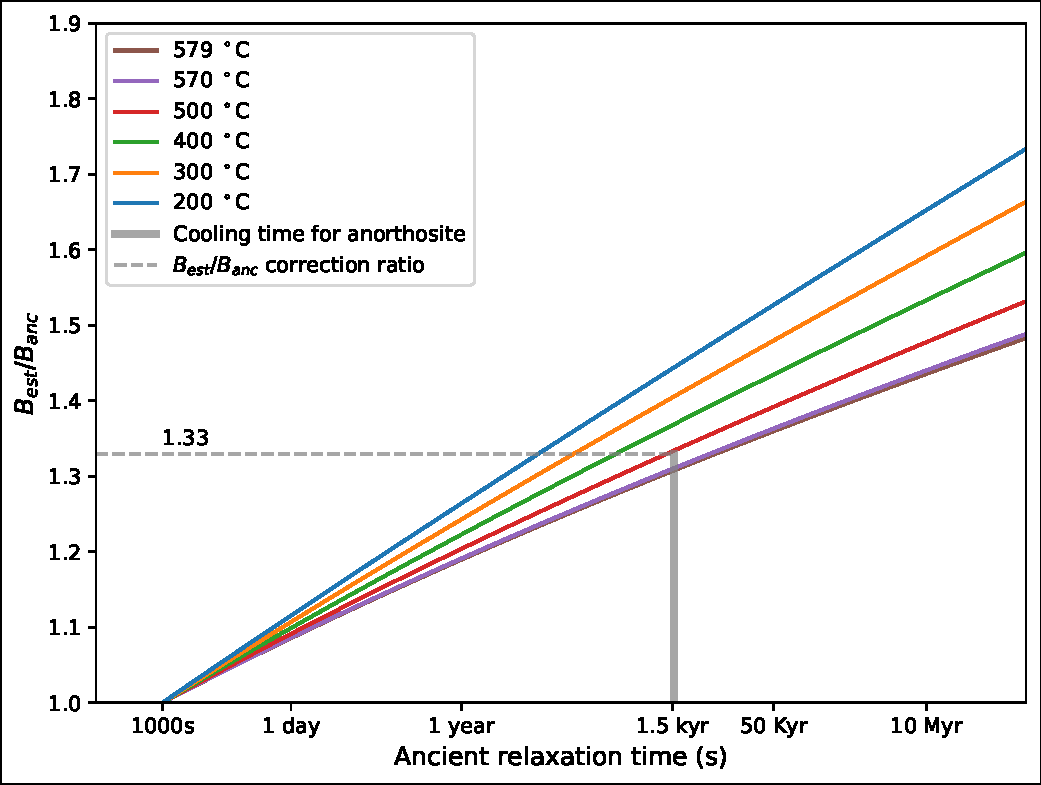
\includegraphics[width=\textwidth]{Cooling_rate_correction.pdf}
% \centering
% \caption{\small{}}
% \label{fig:cooling_correction}
% \end{figure}

% A 20 mT alternating field treatment after in-field heating steps were applied to some specimens in an attempt to mitigate non-ideal behavior contributed by multidomain or non-uniformly magnetized magnetic carriers. The treatment did not make any diabase specimen to pass the selection criteria. On the other hand, 27 out of 58 ($\sim$46.6\%) anorthosite specimens that had AF treatment passed selection and 13 out of 28 ($\sim$46.4\%) specimens without AF treatment passed selection. Paleointensity estimates from specimens with or without AF treatment in anorthosite AX10, AX11, AX12, AX13, AX16 do not show significant difference (Fig. \ref{fig:PINT_cooling_corrected}). Specimen results for AX11 particularly illustrates a case where all specimens within the site yield almost the same paleointensity estimate, regardless of the AF treatment.

% Therefore, the alternating field demagnetization did not result in significant increase in specimen success rate for the anorthosites although it might have improved the specimen behavior for those anorthosites that were subjected to this treatment. Together with the narrow range of unblocking temperatures of their sister specimens \cite{Zhang2021b}, these data are consistent with the interpretation that the anorthosites with successful paleointensity results have a magnetic mineral assemblage that is likely dominated by single domain, low-Ti magnetite. Some anorthosite specimens and all diabase specimens still failed during result selections even though AF treatment was applied. It could be that they have a very high dominance of multidomain (MD) or vortex state grains with relatively moderate coercivity such that an alternating field with 20 mT peak field did not significantly mitigate their non-ideal paleointensity behaviors. Another cause for their failure could be the thermochemical alterations that happened during heating in air. As can be exampled by the zigzagging high temperature slope with poor pTRM checks in paleointensity plot for specimen BD2-5b (Fig. \ref{fig:IZZI_examples}), the decrease in NRM/TRM ratios during higher temperature steps likely resulted from the formation of new ferromagnetic material within the specimen due to oxidation. Such alterations can allow specimens to acquire additional remanence during in-field steps that may not be fully removed by an AF treatment. 

% Further, we applied full TRMs to the anorthosite specimens that pass the paleointensity selection criteria after paleointensity experiment. With an applied field of 30 $\mu$T oriented toward the specimen at 0, 30, 60, 90, 120, and 150 degrees, the anorthosite specimens usually acquired consistent full TRMs. The most significant variations observed in acquired full TRMs reach to only XXX \%, much less than that has been reported to occurred within layerd anorthositic rocks in Stillwater (up to $\sim$60 \%, \cite{Selkin2000a}). 

% Ref. \citealp{Selkin2007a} also noted that vortex state magnetic grains and certain single domain particles can produce biased paleointensity estimates due to their acquisition of saturation remanence during laboratory in-field steps. According to the numerical modeling of  \citealp{Selkin2007a}, thermoremanent magnetization acquired by a population of randomly-oriented, elongate, single-domain magnetite particles are unlikely to saturate upon our applied field of 30 $\mu$T. Therefore, in this study we do not correct for anisotropy or nonlinear TRM to our specimens.

% We applied full TRMs to our anorthosite specimens with lab fields of 30, 50, 70, and 90 $\mu$T along specimen vertical axis. The results show that our anorthosite specimens did not saturate upon an applied field of 30 $\mu$T and there is thus no need for correcting nonlinear thermal remanence acquisitions. 
% Further, we applied full TRMs to the anorthosite specimens that pass the paleointensity selection criteria after paleointensity experiment. With an applied field of 30 $\mu$T oriented toward the specimen at 0, 30, 60, 90, 120, and 150 degrees, the anorthosite specimens usually acquired consistent full TRMs. The most significant variations observed in acquired full TRMs reach to only XXX \%, much less than that has been reported to occurred within layerd anorthositic rocks in Stillwater (up to $\sim$60 \%, \cite{Selkin2000a}). 

% The reason that the Beaver River anorthosite xenoliths do not display strong remanence anisotropy, nor do they display nonlinear TRM acquisition problem, could be that they formed in a magmatic setting distinct from that of a layered mafic complex such as the nearby Duluth Complex, where igneous foliation can occur (Fig. \ref{fig:Geologic_map}). Petrographic images show that an equigranular texture where equidimensional, randomly oriented plagioclase often develop in the anorthosite xenoliths (Fig. \ref{fig:Petro_QDM}; \cite{Zhang2021b}). This is in contrast to the interlocking igneous foliation texture within the Anorthositic Series rocks of the ca. 1096 Ma Duluth Complex (Fig. \ref{fig:Petro_QDM}). Further, petrographic and magnetic imaging also shows the Beaver River anorthosite xenoliths do not develop abundant exsolved magnetite and ilmenite needles within plagioclase crystals as the slowly-cooled anorthositic intrusions do, in which exsolved magnetite needles can be the dominate remanence carriers (Fig. \ref{fig:Petro_QDM}; \cite{Scofield1986a, Feinberg2006a}). The fact that all dipole features within a same Duluth Complex plagioclase crystal have indistinguishable orientations is consistent with the interpretation of there being a magnetic remanence anisotropy resulting from preferred petrofabric alignment, which could give rise to the remanence anisotropy and nonlinear TRM acquisition of layered anorthositic intrusions (Fig. \ref{fig:Petro_QDM}). 